% This is "sig-alternate.tex" V2.1 April 2013
% This file should be compiled with V2.5 of "sig-alternate.cls" May 2012
%
% This example file demonstrates the use of the 'sig-alternate.cls'
% V2.5 LaTeX2e document class file. It is for those submitting
% articles to ACM Conference Proceedings WHO DO NOT WISH TO
% STRICTLY ADHERE TO THE SIGS (PUBS-BOARD-ENDORSED) STYLE.
% The 'sig-alternate.cls' file will produce a similar-looking,
% albeit, 'tighter' paper resulting in, invariably, fewer pages.
%
% ----------------------------------------------------------------------------------------------------------------
% This .tex file (and associated .cls V2.5) produces:
%       1) The Permission Statement
%       2) The Conference (location) Info information
%       3) The Copyright Line with ACM data
%       4) NO page numbers
%
% as against the acm_proc_article-sp.cls file which
% DOES NOT produce 1) thru' 3) above.
%
% Using 'sig-alternate.cls' you have control, however, from within
% the source .tex file, over both the CopyrightYear
% (defaulted to 200X) and the ACM Copyright Data
% (defaulted to X-XXXXX-XX-X/XX/XX).
% e.g.
% \CopyrightYear{2007} will cause 2007 to appear in the copyright line.
% \crdata{0-12345-67-8/90/12} will cause 0-12345-67-8/90/12 to appear in the copyright line.
%
% ---------------------------------------------------------------------------------------------------------------
% This .tex source is an example which *does* use
% the .bib file (from which the .bbl file % is produced).
% REMEMBER HOWEVER: After having produced the .bbl file,
% and prior to final submission, you *NEED* to 'insert'
% your .bbl file into your source .tex file so as to provide
% ONE 'self-contained' source file.
%
% ================= IF YOU HAVE QUESTIONS =======================
% Questions regarding the SIGS styles, SIGS policies and
% procedures, Conferences etc. should be sent to
% Adrienne Griscti (griscti@acm.org)
%
% Technical questions _only_ to
% Gerald Murray (murray@hq.acm.org)
% ===============================================================
%
% For tracking purposes - this is V2.0 - May 2012

\documentclass{sig-alternate-05-2015}
\usepackage{fixme}
\fxsetup{ status=draft, layout=inline}

\usepackage{booktabs}
\usepackage{hyperref}
\usepackage{cite}

\newcommand{\xhdr}[1]{{\vspace{6pt}\noindent\textbf{\textit{#1}}}}
\newcommand{\etal}{~\textit{et al. }}
\newcommand{\etc}{~\textit{etc.}}
\setcounter{secnumdepth}{3} 

\begin{document}

% Copyright
\setcopyright{acmcopyright}
%\setcopyright{acmlicensed}
%\setcopyright{rightsretained}
%\setcopyright{usgov}
%\setcopyright{usgovmixed}
%\setcopyright{cagov}
%\setcopyright{cagovmixed}

%%%%%%%%%%%%%%%%%%%%%%%%%%%%%%%%%%%%%%%%%%%%%%%%%%%%%%%%
%%%% DOI
%%%\doi{10.475/123_4}
%%%
%%%% ISBN
%%%\isbn{123-4567-24-567/08/06}
%%%
%%%%Conference
%%%\conferenceinfo{PLDI '13}{June 16--19, 2013, Seattle, WA, USA}
%%%
%%%\acmPrice{\$15.00}
%%%
%%%%
%%%% --- Author Metadata here ---
%%%\conferenceinfo{WOODSTOCK}{'97 El Paso, Texas USA}
%%%%\CopyrightYear{2007} % Allows default copyright year (20XX) to be over-ridden - IF NEED BE.
%%%%\crdata{0-12345-67-8/90/01}  % Allows default copyright data (0-89791-88-6/97/05) to be over-ridden - IF NEED BE.
%%%% --- End of Author Metadata ---
%%%%%%%%%%%%%%%%%%%%%%%%%%%%%%%%%%%%%%%%%%%%%%%%%%%%%%%%

\title{What's the nature world like behind Flickr?}
%Aggregating Visual Evidence from Social Media Photos to Monitor the Natural World}
%%%Format\titlenote{(Produces the permission block, and
%%%copyright information). For use with
%%%SIG-ALTERNATE.CLS. Supported by ACM.}}
%%%\subtitle{[Extended Abstract]
%%%\titlenote{A full version of this paper is available as
%%%\textit{Author's Guide to Preparing ACM SIG Proceedings Using
%%%\LaTeX$2_\epsilon$\ and BibTeX} at
%%%\texttt{www.acm.org/eaddress.htm}}}

%
% You need the command \numberofauthors to handle the 'placement
% and alignment' of the authors beneath the title.
%
% For aesthetic reasons, we recommend 'three authors at a time'
% i.e. three 'name/affiliation blocks' be placed beneath the title.
%
% NOTE: You are NOT restricted in how many 'rows' of
% "name/affiliations" may appear. We just ask that you restrict
% the number of 'columns' to three.
%
% Because of the available 'opening page real-estate'
% we ask you to refrain from putting more than six authors
% (two rows with three columns) beneath the article title.
% More than six makes the first-page appear very cluttered indeed.
%
% Use the \alignauthor commands to handle the names
% and affiliations for an 'aesthetic maximum' of six authors.
% Add names, affiliations, addresses for
% the seventh etc. author(s) as the argument for the
% \additionalauthors command.
% These 'additional authors' will be output/set for you
% without further effort on your part as the last section in
% the body of your article BEFORE References or any Appendices.

\numberofauthors{3} %  in this sample file, there are a *total*
% of EIGHT authors. SIX appear on the 'first-page' (for formatting
% reasons) and the remaining two appear in the \additionalauthors section.
%
\author{
%%%% You can go ahead and credit any number of authors here,
%%%% e.g. one 'row of three' or two rows (consisting of one row of three
%%%% and a second row of one, two or three).
%%%%
%%%% The command \alignauthor (no curly braces needed) should
%%%% precede each author name, affiliation/snail-mail address and
%%%% e-mail address. Additionally, tag each line of
%%%% affiliation/address with \affaddr, and tag the
%%%% e-mail address with \email.
%%%%
%%%% 1st. author
%%%\alignauthor
%%%Ben Trovato\titlenote{Dr.~Trovato insisted his name be first.}\\
%%%       \affaddr{Institute for Clarity in Documentation}\\
%%%       \affaddr{1932 Wallamaloo Lane}\\
%%%       \affaddr{Wallamaloo, New Zealand}\\
%%%       \email{trovato@corporation.com}
%%%% 2nd. author
%%%\alignauthor
%%%G.K.M. Tobin\titlenote{The secretary disavows
%%%any knowledge of this author's actions.}\\
%%%       \affaddr{Institute for Clarity in Documentation}\\
%%%       \affaddr{P.O. Box 1212}\\
%%%       \affaddr{Dublin, Ohio 43017-6221}\\
%%%       \email{webmaster@marysville-ohio.com}
%%%% 3rd. author
%%%\alignauthor Lars Th{\o}rv{\"a}ld\titlenote{This author is the
%%%one who did all the really hard work.}\\
%%%       \affaddr{The Th{\o}rv{\"a}ld Group}\\
%%%       \affaddr{1 Th{\o}rv{\"a}ld Circle}\\
%%%       \affaddr{Hekla, Iceland}\\
%%%       \email{larst@affiliation.org}
%%%\and  % use '\and' if you need 'another row' of author names
%%%% 4th. author
%%%\alignauthor Lawrence P. Leipuner\\
%%%       \affaddr{Brookhaven Laboratories}\\
%%%       \affaddr{Brookhaven National Lab}\\
%%%       \affaddr{P.O. Box 5000}\\
%%%       \email{lleipuner@researchlabs.org}
%%%% 5th. author
%%%\alignauthor Sean Fogarty\\
%%%       \affaddr{NASA Ames Research Center}\\
%%%       \affaddr{Moffett Field}\\
%%%       \affaddr{California 94035}\\
%%%       \email{fogartys@amesres.org}
%%%% 6th. author
%%%\alignauthor Charles Palmer\\
%%%       \affaddr{Palmer Research Laboratories}\\
%%%       \affaddr{8600 Datapoint Drive}\\
%%%       \affaddr{San Antonio, Texas 78229}\\
%%%       \email{cpalmer@prl.com}
}
%%%% There's nothing stopping you putting the seventh, eighth, etc.
%%%% author on the opening page (as the 'third row') but we ask,
%%%% for aesthetic reasons that you place these 'additional authors'
%%%% in the \additional authors block, viz.
%%%\additionalauthors{Additional authors: John Smith (The Th{\o}rv{\"a}ld Group,
%%%email: {\texttt{jsmith@affiliation.org}}) and Julius P.~Kumquat
%%%(The Kumquat Consortium, email: {\texttt{jpkumquat@consortium.net}}).}
%%%\date{30 July 1999}
%%%% Just remember to make sure that the TOTAL number of authors
%%%% is the number that will appear on the first page PLUS the
%%%% number that will appear in the \additionalauthors section.

\maketitle
\begin{abstract}
Social photo-sharing websites collect a huge amount of latent visual
information about the world, including information about the
environment and ecology. In this work, we propose to reconstruct
satellite maps of environmental status across North America through
millions of publicly available geo-temporal tagged images. We apply
modern deep learning-based recognition techniques to identify
phenomena in images, and then aggregate evidence from multiple users
to estimate whether or not the phenomena were occurring in a given
time and place. We then evaluate the accuracy of these estimates by
comparing to actual satellite maps as ground truth. As test cases, we
consider two important ecological phenomena for which high quality
ground truth is available: snowfall coverage and vegetation (greenery)
coverage. We find that while the automatic recognition techniques are
noisy on any single particular image, we can accurately estimate the
phenomena's presence when enough users have uploaded enough photos at
a particular time and place. This evidence from photo-sharing websites
could create new sources of data for ecologists, perhaps helping to
overcome the limitations of traditional data collection techniques
like manual observation (which is labor intensive) or satellites
(which are not able to observe through clouds).
\end{abstract}


%
% The code below should be generated by the tool at
% http://dl.acm.org/ccs.cfm
% Please copy and paste the code instead of the example below. 
%
%%%\begin{CCSXML}
%%%<ccs2012>
%%% <concept>
%%%  <concept_id>10010520.10010553.10010562</concept_id>
%%%  <concept_desc>Computer systems organization~Embedded systems</concept_desc>
%%%  <concept_significance>500</concept_significance>
%%% </concept>
%%% <concept>
%%%  <concept_id>10010520.10010575.10010755</concept_id>
%%%  <concept_desc>Computer systems organization~Redundancy</concept_desc>
%%%  <concept_significance>300</concept_significance>
%%% </concept>
%%% <concept>
%%%  <concept_id>10010520.10010553.10010554</concept_id>
%%%  <concept_desc>Computer systems organization~Robotics</concept_desc>
%%%  <concept_significance>100</concept_significance>
%%% </concept>
%%% <concept>
%%%  <concept_id>10003033.10003083.10003095</concept_id>
%%%  <concept_desc>Networks~Network reliability</concept_desc>
%%%  <concept_significance>100</concept_significance>
%%% </concept>
%%%</ccs2012>  
%%%\end{CCSXML}
%%%
%%%\ccsdesc[500]{Computer systems organization~Embedded systems}
%%%\ccsdesc[300]{Computer systems organization~Redundancy}
%%%\ccsdesc{Computer systems organization~Robotics}
%%%\ccsdesc[100]{Networks~Network reliability}
%%%
%%%
%%%%
%%%% End generated code
%%%%
%%%
%%%%
%%%%  Use this command to print the description
%%%%
%%%\printccsdesc

% We no longer use \terms command
%\terms{Theory}

\keywords{social media mining; computer vision; scene recognition}

\section{Introduction}

Monitoring the state of the natural world is a key challenge of
ecological and biological research, since predicting future changes
depends on accurate observations of the present. Satellites give
observations at large scale but can only be applied to phenomena that
can be seen from far above, and are limited by cloud cover and other
atmospheric conditions.  Citizen science projects~\cite{citizensci} can
produce quality data, but require significant incentives to encourage
participation over large scale areas, and clever designs to derive
accurate data from untrained observers.  A potentially rich
alternative is to mine publicly-available social media for
observations relevant to natural world, in effect turning the billions
of social media users into citizen scientists without any explicit
actions on their part.  This idea is motivated by the large amount of
work that has  mined social media  to predict and
observe properties of the real world, including the stock
market~\cite{bollen11twitter},
elections~\cite{you2015multifacetedelections}, tourism
activity~\cite{wood2013usingtourism}, and so on.

However, most of this work has used textual data like Facebook posts
and Twitter feeds.  Social images are potentially a richer source of
information because they often include incidental evidence about the
natural world (Figure~\ref{fig:flickrexp}).  In addition, they record
visual documentation that can later be analyzed, inspected, and
validated; the danger of relying on text analysis and the importance
of validation was recently recently illustrated by the case of Google
Flu, which initially showed great promise in monitoring the spread of
influenza by mining search engine queries~\cite{ginsberg09flu}, but
was later found to be largely inaccurate~\cite{lazer2014parable}.
Of course, a key challenge in mining images is how to extract useful
semantic information.

\begin{figure}[t]
{\tiny{
\begin{center}
\begin{tabular}{@{}c@{\,\,\,}c@{\,\,\,}c@{\,\,\,}c@{\,\,\,}c@{\,\,\,}c@{\,\,\,}c@{\,\,\,}c@{\,\,\,}}
%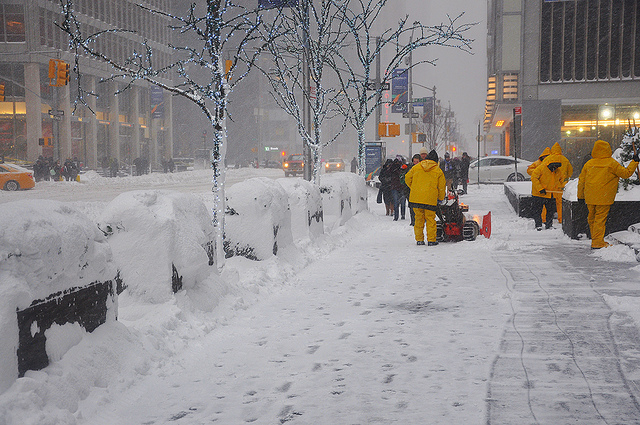
\includegraphics[width=0.12\textwidth]{image/citysnow.jpg} &
%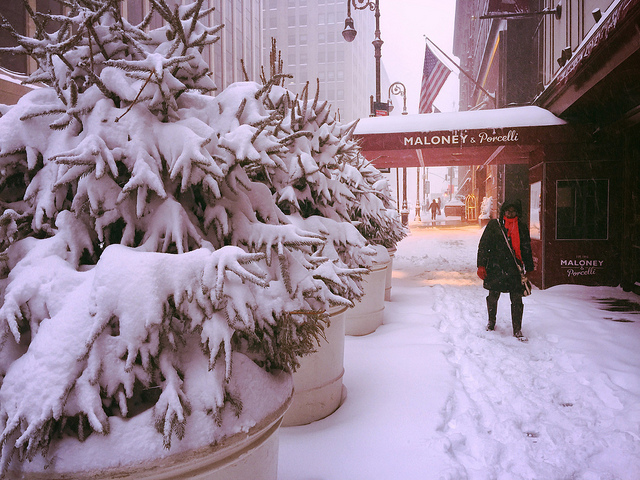
\includegraphics[width=0.1\textwidth]{image/citysnow2.jpg} &
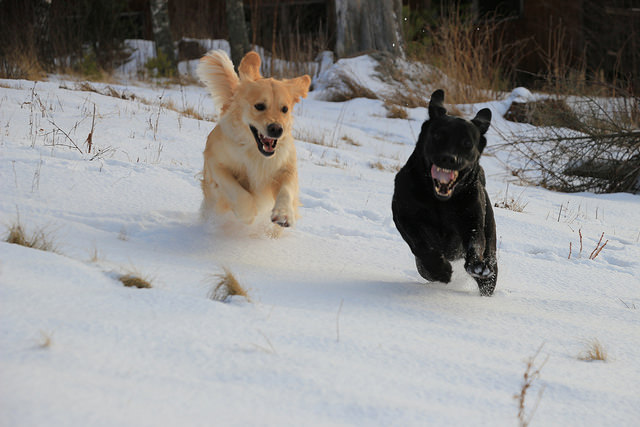
\includegraphics[width=0.15\textwidth,height=0.75in]{image/dogsnow.jpg} &
%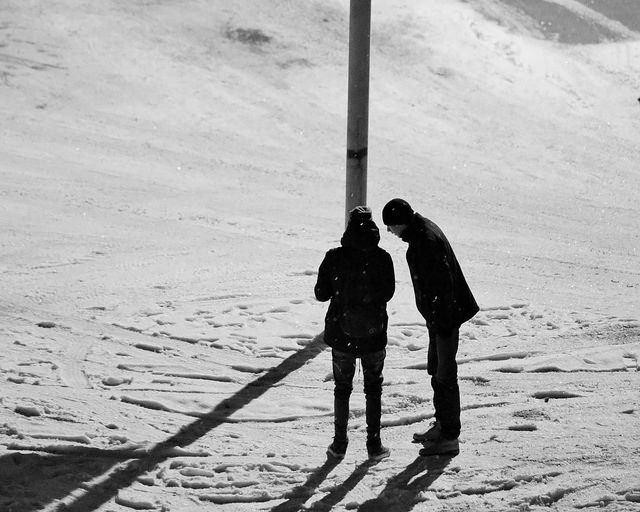
\includegraphics[width=0.1\textwidth]{image/humansnow.jpg} \\
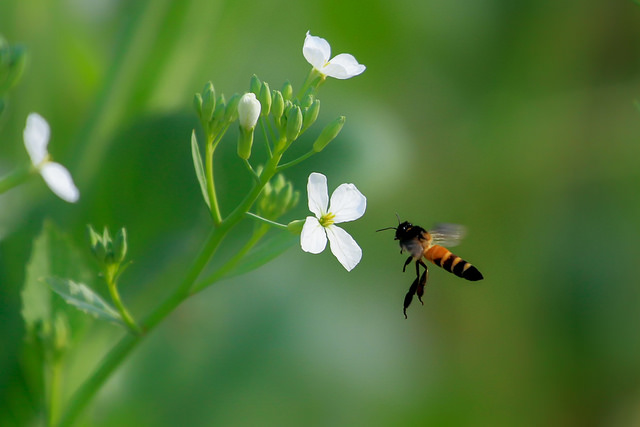
\includegraphics[width=0.15\textwidth,height=0.75in]{image/intentiongreen.jpg} &
%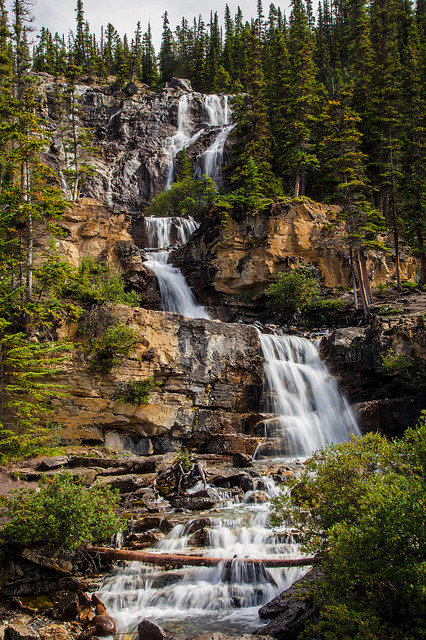
\includegraphics[width=0.1\textwidth]{image/waterfallgreen.jpg} &
%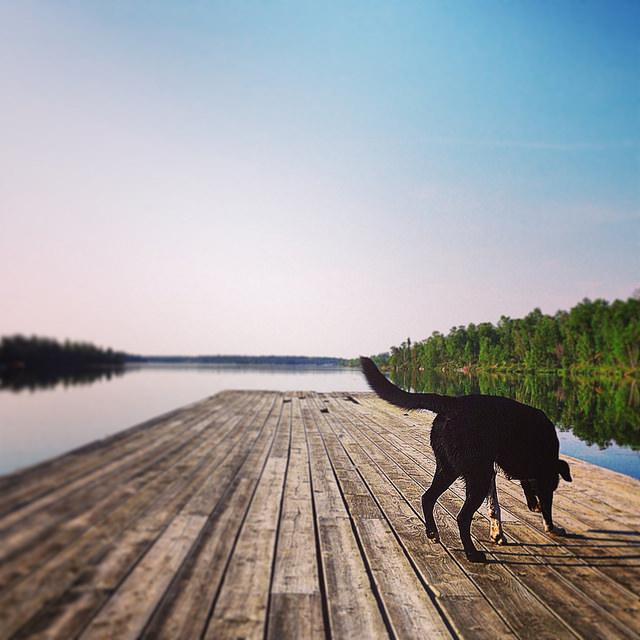
\includegraphics[width=0.12\textwidth,trim=0 0 0 cm,clip]{image/dogtree.jpg} &
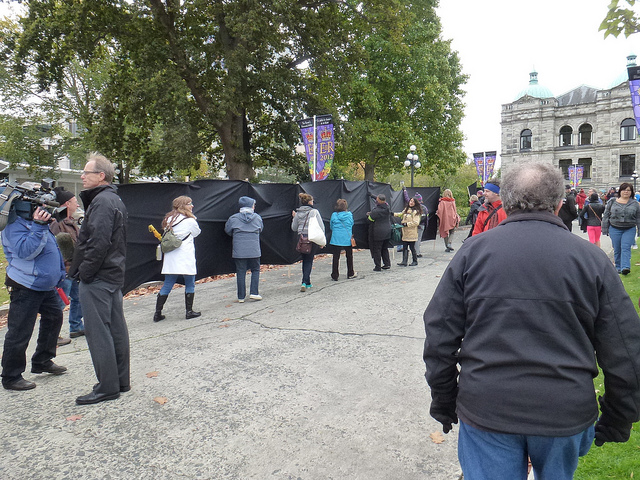
\includegraphics[width=0.15\textwidth,height=0.75in]{image/humantree.jpg} \\
\end{tabular}
\end{center}
}}
\vspace{-12pt}
\caption{Many social media images capture information about the state of the natural world, both intentionally or incidentally.}
\label{fig:flickrexp}
\vspace{-12pt}
\end{figure}


A few papers have begun to apply computer images for environmental
properties, including temperature~\cite{glasner2015hot}, cloud
cover~\cite{murdock2013webcam2satellite}, and smog conditions~\cite{li2015smog}. Most of
these papers use video data (e.g.\ from static webcams) so that visual
changes over time can be easily detected. Video camera feeds are
potentially very useful for studying longitudinal changes across time
in one particular place, but are limited to studying places where
cameras have been installed. Social photo sharing websites potentially
represent a complementary source of data, that give much greater
spatial coverage: whenever a user takes a photo at a particular place
and time and uploads it to Flickr, they are contributing a potentially
useful observation.

In this paper, we test the feasibility of leveraging these noisy and
biased images as a new source to observe nature, using modern deep
learning-based computer vision algorithms to recognize image content
automatically.  As a case study, we investigate two particular
phenomena, snowfall and vegetation coverage, since they are important
properties of the environment, they are relatively easy to recognize,
occur frequently in social images, and have satellite maps available
to serve as ground truth. This choice was also inspired by Fedorov et
al~\cite{fedorov2015snowwatch,fedorov2014snow}, who use video analysis
to monitor snow fall on mountains, and Zhang et
al~\cite{ecology2012www}, who predict snowfall from image collections
but using text tag analysis.  We first collect image data labeled to
reflect the presence of absence of ecology phenomena, and train
classifiers using Convolutional Neural Networks to recognize these
ecology phenomena in individual images. Of course, these classifiers
are noisy, and social image data is noisy also, with many inaccurate
timestamps and geo-tags.  We thus train an additional classifier that
examines all images taken at a given place and time, runs the image
classifier on each one, and then predicts if the phenomena actually
occured there and then.  Finally, we evaluate at a large scale,
training and testing on millions of Flickr images and quantiatively
evaluating the performance at hundreds of thousands of places and
times.

%% Inspried by an earlier work~\cite{ecology2012www} 
%% %\fxnote{ Fixed: cite{www}} 
%% analyzing ecology phenomenon from image tags only. We apply a new approach by 
%% understanding visual content of images, and run experiments on the exact same 
%% data set to study how vision techniques could help in social media data mining 
%% compared to using textual data alone. Also, to our best knowledge, among all the 
%% research works performing social sensing with image data, this is the first one 
%% providing continental scale quantitative performance evaluation.










\begin{figure}[t]
\centering
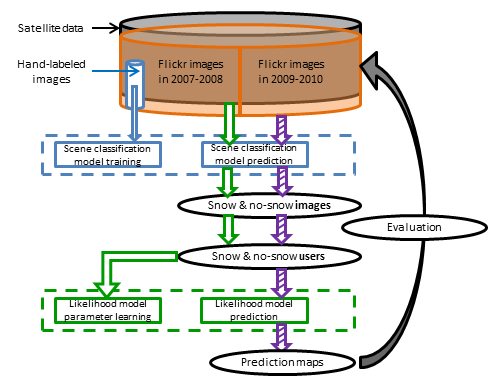
\includegraphics[scale=0.7]{figure/flowchartWevaluation.png}
\vspace{-12pt}
\caption{Overview of our approach. We train image classifiers(in blue) on large scale images. And by applying it to training images in 2007-2008, 
we train a likelihood model(in green) and finally make prediction by aggregating these visual evidence.}
% \fxnote{first classifier, then prediction}
\label{fig:overview}
\vspace{-12pt}
\end{figure}


\section{Related work}
In last few years, crowd-sourcing data from social media 
as a large scale and free to public data source
has \fxnote{received lots of attention from; or (become more and more popular to)} 
researchers working on using textual contents to
predict elections~\cite{you2015multifacetedelections},
using geo-tags to quantify
tourism in nature area using geo-tag profile of social media users ~\cite{wood2013usingtourism},
\fxnote{talk a lot about motivation of scientific report paper since it's in nature area}
to draw coastline~\cite{omori2014can}~\cite{Can geo-tags on flickr draw coastlines?}, 
using geo and temporal tags to analyze people's event-based activity when large group of people gathering together during a function of time such as football match,
and using both geo and textual tags to 
extract land use information from Panoramio~\cite{vsecerov2015analysis} ~\cite{Analysis of panoramio photo tags in order to extract land use information, Towards Better Land Cover Classification Using Geo-tagged Photographs},
in~\cite{ecology2012www} \fxnote{cite{www}}, Zhang \etal estimates \fixme{missing letter in compiling} snowfall and vegetation coverage 
based on geo, temporal and textual tags of Flickr images. \fxnote{accuracy of geo-temporal problem, and now it's getting better.}

Since public-sharing photos provides such a huge potential in social and environmental study, it's 
natural to see a lot of works start analyzing image contents. Webcam providing dense temporal images 
is a good source to monitor the nature. A series of works explore sequences 
of webcam images describing outdoor scene with 40 transient attributes~\cite{transattri}, estimating dynamic cloud maps ~\cite{murdock2015building, murdock}, exploring interactions between visual elements and the temperature \fxnote{or just as the title: exploring correlations between appearance and temperature} ~\cite{hot or not}, and monitoring the dynamic snow phenomena at mountain areas ~\cite{fedorov2015snowwatch, fedorov2014snow}. 
To evaluate the study of temperature, cloud, and snowfall amount,
 researchers can easily compare their results with satellite maps. 
Some works also use crowd-sourcing data from other sources, for example, Google street view provides selectively dense geo distributed images to help navigating the environment ~\cite{khosla2014looking} and understanding urban scene and predicting urban perception ~\cite{porzi2015predicting}, and Li \etal use the co-occurrence statistics of celebrities appears on news images to auto tag photographs of celebrity community ~\cite{li2015celebritynet}
\fxnote{give a term like social identity?}. 
Unfortunately, 
the evaluation in these works are either not in continental scale or just via quality visualization.
Performance of social activity studies, on the other hand, are even harder to evaluate.
\fxnote{say more about our evaluation? or move this to another place?}

Flickr and Panoramio as very popular photo-sharing websites 
``involuntarily'' support researchers identifying salient city attributes and analyzing the visual similarity among different cities in order to apply computer vision to urban planning ~\cite{zhou2014recognizing}
Photo-sharing websites collecting visual contents directly from people's activity and their surrounding areas which is so important, hard to collect otherwise but also very noisy. \fxnote{write something about so there are very few work appears and so we are working on this?}

%\fxnote{not sure about keeping this paragraph or not. it seems duplicate of the 2 paragraphs above}

The fact that webcam can only be placed far away from people 
 makes it almost impossible to monitor people's activity, even not the surrounding area close to
residential or \fxnote{crowd? I mean groups of people like downtown, not ski activity but like people 
going to work and back everyday also a good topic to use temporal dense images but Webcam is not good 
at this.} Social media, on the other hand, provides a larger freedom on location distribution. 
In fact, as a complementary, almost all the photos shared online are from locations people usually go to. 
\fxnote{how helpful is this to study more areas close to urban planning, market sharing, everyday living,
anything related to people}

Our work take the advantage of studying ecology phenomena with \fxnote{easy to get, more reliable} satellite maps as
 ground truth and use social media data to \fxnote{monitor? insight?} these information from \fxnote{
locations more related to people}. We provide continental scale quantitative evaluation and introduce our
 method to tackle the problem of noisy and biased data, in order to support extended studies in other areas. \fxnote{just want to say more areas in natural or not only natural but also social}


%\section{method}

\subsection{Overview}
In this paper, we propose an effective system to estimate the presence or absence 
of a given ecology phenomenon (like green leaf plants) 
from visual contents of public-shared photographs. First, we employ the state-of-the-art 
computer vision technique to detect the target phenomenon. Then according to the visual evidence 
and the corresponding timestamp and geo-tag of each image, we use a likelihood model 
aggregating the large scale, imperfect information to reconstruct the satellite maps.

We collect 12 million photos shared on Flickr during 2007 and 2010 with geo-tags and timestamp available, 
in North America continent similar to \fxnote{cite{www}}, and split them into a training set $D_1$ for prior knowledge 
learning with photos taken in 2007 and 2008, and a testing set $D_2$ with photos taken in 2009 and 2010.
In the two steps of training stage, for snowfall and greenery respectively, we first 
prepare a hand-labeled dataset similar to 
\fxnote{cite{workshop}} sampled from photos taken 
before 2009, no matter it has geo or temporal 
information or not. Half of the photos must have tags indicating snow or greenery presenting 
in the image as positive samples, and the other half are random negative samples. 
We learn a scene classification model from this hand-labeled dataset for each target phenomenon. By  
applying this model to the continental scale dataset $D_1$, in the second step 
of training, we learn the parameters for the likelihood model introducing later 
in \fxnote{section 3.3} to 
make estimation for each pixel on our result map. We then test the entire system with the separate continental 
scale dataset $D_2$ and compare the results with satellite maps described in \fxnote{cite{www}} as ground 
truth for evaluation.

\subsection{Scene Classification}
\subsubsection{Combining Visual Features}
To train a scene classification model for snow scene and greenery scene respectively, we start with 
combining the most discriminative image features. Similar to snow scene recognition in \fxnote{cite{workshop}}, 
vegetation has the signature green color that the  
biologists are very interested in during exactly which time period they are green. 
Thus it's very important 
to find out when it turns from yellow to green and when does it turns back to yellow.
The leaves of plants also have distinctive visual texture. 
Thus, visual features capture both color and texture information are our best choice.
So we employ color SIFT feature \fxnote{cite{SIFT}} to analyze the local gradient distribution. 
And we also extract color GIST feature to describe texture feature and global context. 

\xhdr{Color SIFT histogram.}
We extract dense SIFT feature on each of the RGB color plane, and concatenate them to 
build color SIFT feature. The dense SIFT feature is extracted from every 2 pixels by 2 pixels bin, 
with a step size of 5 pixels. In this way, we achieve representative key points and reasonable 
computation complex. 

From training data set, We build 2000 dimensional centers of color SIFT feature 
using K-means clustering. With these centers, a 2000 dimensional histogram is built 
from all the key points of each image.

\xhdr{Color GIST.} Similarly, we also extract GIST features on RGB color channel respectively.
\fxnote{From now on to the end of this paragraph, 
it's the same as our workshop paper. Could you help me to give a shorter global
description?}
GIST feature capture coarse texture
and scene layout by applying a Gabor filter bank followed by
down-sampling \fxnote{cite{oliva2001modeling}}. Our variant produces a
1536-dimensional vector and operates on color planes. Scaling
images to have square aspect ratios before computing GIST improved
classification results significantly \fxnote{cite{douze2009evaluation}}.

By concatenating color SIFT histogram and color GIST feature, 
a model is trained and tested with SVM using RBF kernel.

\subsubsection{Deep learning}
Recently the Conventional Neural Network (CNN) \fxnote{cite{krizhevsky2012imagenet} }
has gained a lot of attention 
in the vision community, as it outperformed all other techniques in the ImageNet challenge 
(the most famous object category detection competition) \fxnote{cite{ilsvrcarxiv14}}.

CNN is currently the state-of-the-art algorithm of image classification on standard datasets.
CNN enjoys additional features that distinguish it from the standard neural networks: 
shared weights and sparse connectivity.
A layer in CNN may consist of three different stages: 
convolution, non-linear activation, and pooling.
In the convolution stage, a set of convolution filters is applied in parallel. 
The output of a convolution filter is then passed to non-linear activation functions 
(e.g., rectified linear activation function, sigmoid activation function).
The final stage is pooling, where the net output is manipulated based on its neighbors 
(e.g., max pooling, $L_2$ norm, and weighted average).
Pooling makes the network invariant to the translation of the input

The key idea behind this approach is that instead of first designing low-level features by
hand and then running a machine learning algorithm, a single unified
algorithm should learn both the low-level features and the
high-classifier simultaneously. 

We apply CNN to detect snow and vegetation on image level. 
We followed \fxnote{cite{Oquab14}} and started with a model pre-trained on the huge 
ImageNet dataset then we train our models using hand-labeled data sets.

\subsection{Aggregating Visual Evidence Across Users}
After image classification, we could have simply count how many photos have evidence of snowfall 
or greenery in the content taken in a given time period at a given place. But, in fact, while we are 
enjoying millions of free and public images on social media websites, we are facing the following problems 
at the same time. The photographers upload these images completely for their own social and personal purposes. 
They may upload a large batch of images without any evidence of our target scene, for example, 
on a snow 
day, people can still upload hundreds of indoor photos or close up photos of their dogs or kids or plants 
in their cleaned backyard. 
Or simply due to device setting of the camera or smartphone, and sometimes limited GPS accuracy of the photographing 
device and satellite, it's possible 
to have a photographer uploading a large number of images with incorrect timestamp or geo-tag.
In this case, which is likely to see on social media websites, we count the visual evidence 
by users instead of by images.

We adopt the likelihood model from \fxnote{cite{www}}, by applying the scene classification model 
to the training dataset $D_1$, we figure out for each location during each time period which image
is 
capturing the target scene (snowfall or greenery) and which is not. For the remaining description, 
we use snowfall as our target scene as an example. First, by combining the 
user profile of each image, we count the number of users denoting in $m$ providing evidence of 
snowfall (event $u$), and 
the number of users denoting in $n$ uploading photos without snowfall (event $\bar{u}$). We learn a 
fixed probability of when satellite map shows it's a snow day at a given location, we see a 
photographer 
uploading images contain snowfall $p = P(u|snow)$. Similarly, $q = P(s | \overline{snow})$ denotes 
the 
probability of when we find a photographer sharing images with snowfall evidence but 
satellite map shows it's not snowing at that time and location. We assume $q$ is a non-zero probability 
due to misleading visual contents (photos with very bright wall or a small chance of false positive 
result from scene classification), and inaccurate geo and temporal tags.

According to \fxnote{cite{www}}, assuming users are taking photos independently, 
given all observers (photographers) spotting snow 
or non-snow, we have the posterior probability of snowfall presence at each time and location:
%
%
\newcommand{\smsn}{s^m, \bar{s}^n}
\newcommand{\smsntwo}{s^m, \bar{s}^n}
%
\begin{eqnarray*}
P(snow|\smsn) &=&\frac{ P(\smsn|snow)P(snow)}{P(\smsntwo)} \\
&=&\frac{{m+n\choose m}p^{m}(1-p)^{n}P(snow)}{P(\smsntwo)}, 
\end{eqnarray*}
%
where we use $P(snow)$ as a general prior probability describing in entire North America, 
the chance to see a snow day at 
any time of a year. So we can also derive the similar posterior probability for absence of snowfall,
%
\begin{eqnarray*}
P(\overline{snow}|\smsn) &=&\frac{{m+n\choose m}q^{m}(1-q)^{n}P(\overline{snow})}{P(\smsntwo)}. 
\end{eqnarray*}
%
We derive the likelihood score by taking the ratio of the snow and non-snow probability.
It can be considered as a measure of the confidence that snow actually appeared at a given time 
and place 
by given all user observations.
%
\begin{eqnarray}
\frac{P(snow|\smsn)}{P(\overline{snow}|\smsntwo)}
&=&\frac{P(snow)}{P(\overline{snow})}\left(\frac{p}{q}\right)^{m}\left(\frac{1-p}{1-q}\right)^n
\label{eq:conf}
\end{eqnarray}



\section{experiments and results}

In this paper, we propose an effective system to estimate the presence or absence 
of a given ecology phenomenon (like green leaf plants) 
from visual contents of public-shared photographs. First, we employ the state-of-the-art 
computer vision technique to detect the target phenomenon. Then according to the visual evidence 
and the corresponding timestamp and geo-tag of each image, we adopt the likelihood model in ~\cite{ecology2012www}
aggregating the large scale, imperfect information to reconstruct the satellite maps.

In Scene classification, we also employ the current state-of-the-art algorithm, 
the Convolutional Neural Network (CNN) pre-trained on ImageNet dataset. 
The key idea behind this approach is that instead of selecting and combining hand designed features 
with limited parameters to fit each recognition task, it learns hierarchical image feature directly 
for target objects.
We fine-tune it with our 
hand-labeled dataset for each experiment case and further improve the performance illustrated below.


We study two important ecology phenomena, for each time period and location, 
whether there is snowfall and are there many plants with green leaves? We discuss the experimental setup 
and the results and evaluation below.

\subsection{Snow Case}
\xhdr{Scene Classification}
%We are using the same hand-labeled dataset as in ~\cite{wang2013observing}.
Beyond combining visual features, 
we build CNN visual model for our snow scene classification problem 
by fine-tuning Imagenet pre-trained model with the 8000 training images labeled for snow scene~\cite{wang2013observing}. The best 
performance in ~\cite{wang2013observing} using visual features with SVM is $80.50\%$ accuracy.
On the same testing set of 2000 images, our CNN model achieves $88.06\%$ accuracy as a significant 
improvement. Details of comparison between performance of CNN model
 and other visual features are presented in Table ~\ref{tab:snow}. Therefore, we use this as our recognition model for final predictions.

Figure ~\ref{fig:PR_ROC_snow} compares classification performance of CNN with 
individual visual features and their combination in terms of an ROC curve, 
as well as a precision-recall curve in which the task is to retrieve photos containing snow.
The precision-recall curve of CNN shows that at about $50\%$ recall, precision is very close to $100\%$, 
while even at $80\%$ recall, precision is still above $90\%$. This is a nice feature because 
in many applications, it may not be necessary to correctly 
classify all images, but instead it is important to find some images that most likely contain snowy 
scene.

We now turn to present experimental results for estimating geo-temporal distributions of snowfall.

\xhdr{Snow Prediction on Cities}
To compare with existing results in ~\cite{wang2013observing} using tag based method,
we first test how well our image-content based method can predict snowfall on daily base at a local scale, 
and in particular 
for the same four U.S. metropolitan areas, New York City, Boston, Chicago and Philadelphia. 
Table~\ref{tab:city_conf_tag_vision} 
shows some basic statistics for these 4 cities, and results of these classifiers. 
Best performance obtained when we combine 
the confidence scores of tags and visual model based on CNN. For each of the method, 
Chicago gives the highest accuracy while Philadelphia gets the lowest accuracy. 
It's reasonable considering that Chicago has the most active Flickr users per
day (94.9) while Philadelphia has the least (43.7). 

There is not a clear evidence that visual evidence is more informative in estimating snowfall 
presence. In contrast, it gets lower accuracy in all these 4 cities. But combining tag and visual 
confidence achieves considerable improvement in performance. We apply this combined model 
in the following experiments.

\xhdr{Continental-scale Snow Prediction}
Adding visual evidence, we reconstruct Satellite maps and 
evaluate our model in continental scale. We follow the same metric in ~\cite{ecology2012www} to produce 
estimation at resolution of $1 \times 1$ degree (roughly $100 \times 100 km^2$) square and get one map for 
each day in 2009 and 2010.

Figure ~\ref{fig:snowcurve} shows the precision and recall curve of snow and non-snow prediction in 
continental-scale.
Here we limit our predictions for the bins which both have photos taken at that 
time and location and have satellite ground truth available.
We computed our confidence scores based on tags and image-classification, then we trained 
simple decision tree to learn the correct thresholds to make final prediction. We achieve 
almost 0.5\% over the baseline (cutting the error rate by more than 20\%), the baseline in 
our case is the majority class which predicts non-snow all the time. 




\vspace{-12pt}
\begin{table}[th!]\centering
\caption{\textbf{Performance of different features for snow detection using SVMs for classification and compared with CNN model.}}
\label{tab:snow}
\tiny
\begin{tabular}{@{}lcr@{}}\toprule
Feature & Kernel & Accuracy\\\midrule
Random Baseline & --- & 50.0\%\\
Gist & RBF & 73.7\%\\
Color  & $\chi^2$ & 74.1\%\\
Tiny & RBF & 74.3\%\\
Spatial Color Moments & RBF & 76.2\%\\
Spatial pyramid LBP & RBF &\textbf{77.0\%}\\\midrule
All features  & linear & \textbf{80.5\%}\\
CNN& -& \textbf{88.1\%}\\
\bottomrule\\
\end{tabular}
\vspace{-8pt}
\end{table}


\begin{figure}[th!]
\begin{center}
\vspace{-16pt}
\begin{tabular}{cc}
 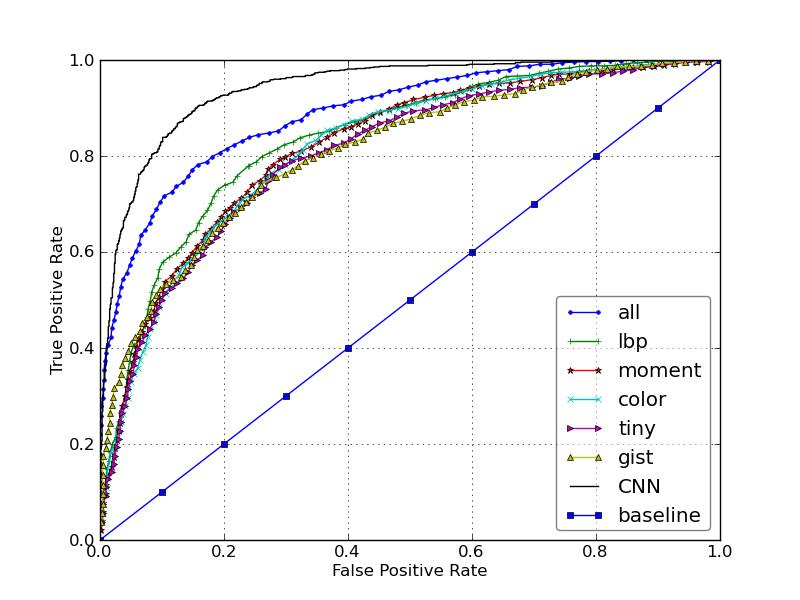
\includegraphics[width=0.2\textwidth]{figure/ROC-CNN-curves.jpg} &
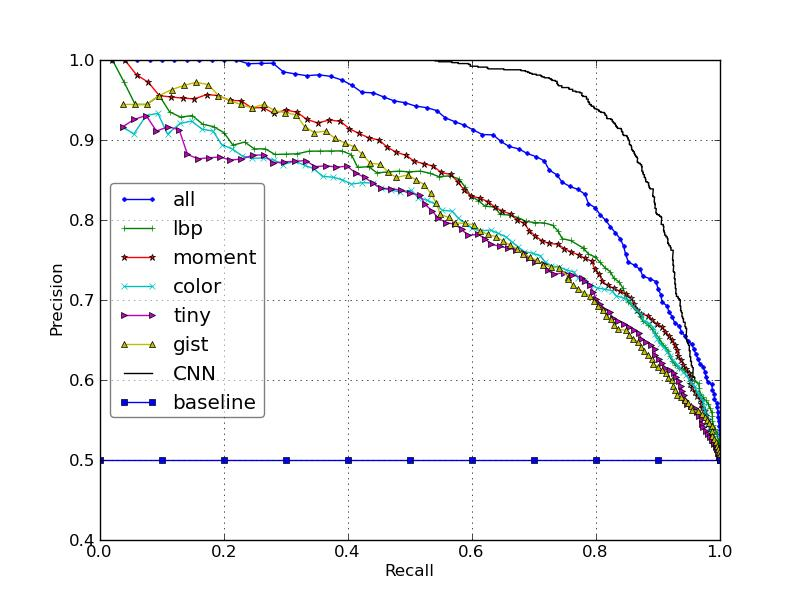
\includegraphics[width=0.2\textwidth]{figure/PR-CNN-curves.jpg} \\
\end{tabular}
\end{center}
\vspace{-24pt}
\caption{
Snow classification results for different features and combination, in terms of {\textit{(left):}} ROC curves for the task of classifying snow vs. non-snow images; and 
{\textit{(right):}} Precision-Recall curves for the task of retrieving snow images.
}
\label{fig:PR_ROC_snow}
\vspace{-8pt}
\end{figure}


\begin{table}[th!]\centering
\caption {\textbf{Selected basic statistics during 2007 to 2010 for the 4 cities and results of the likelihood model using tags and vision evidence.}}
\label{tab:city_conf_tag_vision} 
\tiny
\begin{tabular}{@{}ccccccc@{}}\toprule
City 
& \multicolumn{1}{p{0.2cm}}{\centering naive\\baseline} 
& \multicolumn{1}{p{0.8cm}}{\centering active\\user/day} 
& \multicolumn{1}{p{0.3cm}}{\centering snow\\days} 
&  \multicolumn{1}{p{0.8cm}}{\centering tag\\confidence} 
&  \multicolumn{1}{p{0.7cm}}{\centering vision\\conf} 
& \multicolumn{1}{p{1.4cm}}{\centering tag conf \&\\vision conf} 
\\\midrule
{NYC} & 85.00\% & 65.6 & 185 &90.42\%&90.29\% &92.34\%\\
{Chicago} &72.80\% & 94.9 & 418 &94.12\% &93.16\% &95.08\%  \\
{Boston} & 75.60\%& 59.7 & 373 &89.18\%&85.21\% & 91.23\% \\
{Philly} & 80.50\% & 43.7 & 280 & 89.19\% &85.09\% & 89.19\%  \\
\bottomrule
\end{tabular}
\vspace{-8pt}
\end{table}

\begin{figure}[th!]
\begin{center}
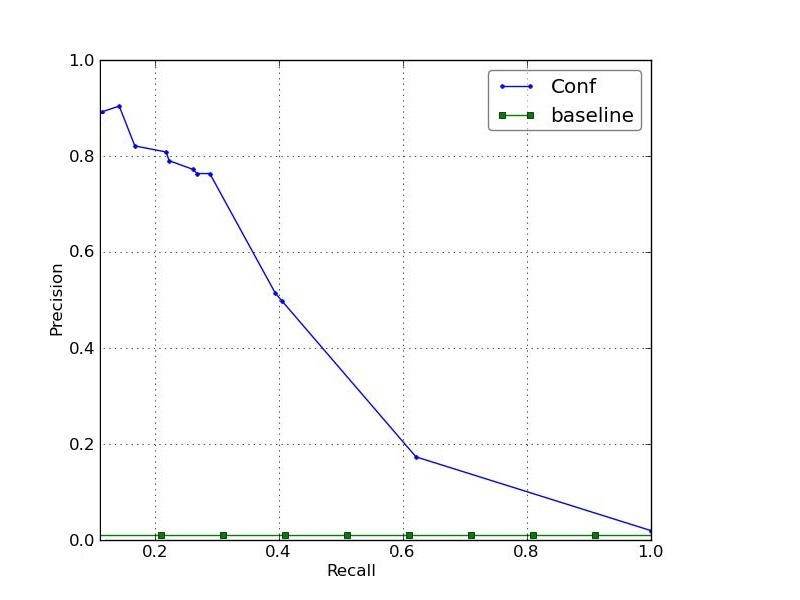
\includegraphics[width=0.18\textwidth,clip,trim=0.4in 0 0.8in 0]{figure/PR-snow.jpg}
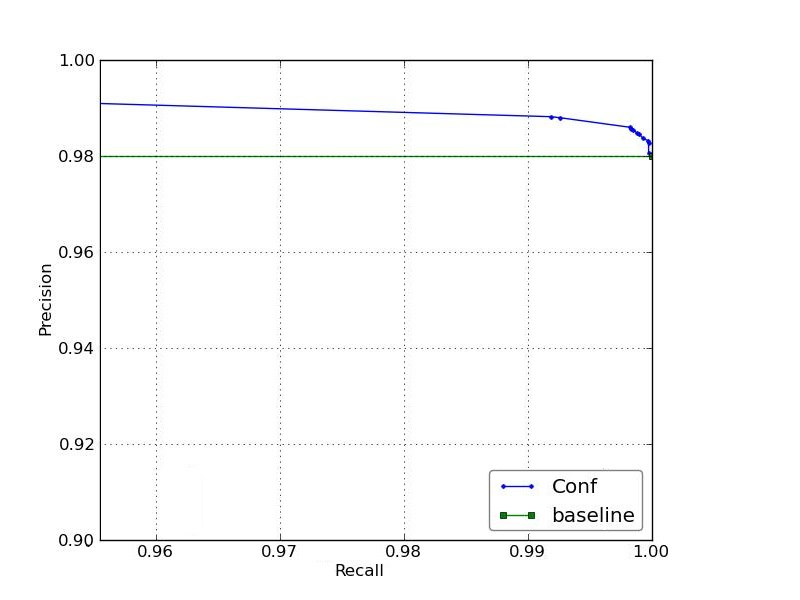
\includegraphics[width=0.18\textwidth,clip,trim=0.4in 0 0.8in 0]{figure/PR-nonsnow.jpg}
\end{center}
\vspace{-24pt}
\caption{Precision and recall curve of snow prediction (left) and nonsnow (right) in continental scale.}
\label{fig:snowcurve}
\vspace{-12pt}
\end{figure}























\subsection{Vegetation Case}

Vegetation coverage is a more stable phenomenon, so we study this case in every 16 days period instead of daily base.
Unlike snow scene that 
tag feature is very discriminative, according 
to ~\cite{ecology2012www}, textual tag of greenery is highly misleading. 
Terms like ``tree'' or even ``leaf'' are not necessarily 
indicating green color, but terms like ``green'' or 
``yellow'' could be used to describe a wild set of objects outside of vegetation. Moreover, while vegetation is 
such a common natural scene appears in most of the outdoor images, it is very unlikely people would include it in their textual tags 
to describe the image. In this case, from a huge number of images contain greenery shared online, only a very small portion of them 
actually provides related textual tags. On the other hand, we believe visual feature can be very descriptive and exclusively 
describing vegetation with green leaves.



\xhdr{Dataset}
We build a data set with over 10000 Flickr images taken before 2009, and are composed by images with "forest" and "summer" like tags 
and also random images without any tag preference. These images are hand labeled with categories 
\textit{"Outdoor Greenery","Outdoor non-Greenery","Indoor","Other-modified"},and \textit{"Not available"}.

Finally, we build a positive set with images in category \textit{"Outdoor Greenery"} and a negative set 
with images in categories \textit{"Outdoor non-Greenery"} and \textit{"Indoor"}. To learn a image classification model, 
we build a training set with 4000 images and a testing set with 1900 images. 
In training and testing set, there are equal number of positive and negative samples.

In continental-scale prediction, we only look at images on Flickr.com in year 2007 to 2010, with no tag limitation. 
We filter out the photos with too unreasonable timestamps such as the taken time and uploading time is exactly the same.
We only use images with high precision geotag according to the image metadata. And we still process the 
satellite ground truth the same way as in ~\cite{ecology2012www}.



\xhdr{Scene Classification}
We hand-labeled a separate dataset for greenery scene.
Compare to snow scene recognition,
vegetation has the signature green color that the  
biologists are very interested in during exactly which time period they are green. 
Thus it's very important 
to find out when it turns from yellow to green and when does it turns back to yellow.
The leaves of plants also have distinctive visual texture. 
Thus, visual features capture both color and texture information are our best choice.
So we employ color SIFT feature to analyze the local gradient distribution. 
And we also extract color GIST feature to describe texture feature and global context. 

\textbf{Color SIFT histogram.}
We extract dense SIFT feature ~\cite{lowe1999object} on each of the RGB color plane, and concatenate them to 
build color SIFT feature. The dense SIFT feature is extracted from every 2 pixels by 2 pixels bin, 
with a step size of 5 pixels. In this way, we achieve representative key points and reasonable 
computation complex. 

From training data set, We build 2000 dimensional centers of color SIFT feature 
using K-means clustering. With these centers, a 2000 dimensional histogram is built 
from all the key points of each image.

\textbf{Color GIST.} Similarly, we also extract GIST features on RGB color channel respectively.
%%%%%%%%%%%%%%%%%%%%%%%%%%%%%%%%%%%%%%%%%%%%%%%%%%%%%%%%%%%%%%%%%
%\fxnote{From now on to the end of this paragraph, 
%it's the same as our workshop paper. Could you help me to give a shorter global
%description?}
GIST feature capture coarse texture
and scene layout by applying a Gabor filter bank followed by
down-sampling ~\cite{oliva2001modeling}. Our variant produces a
1536-dimensional vector and operates on color planes. Scaling
images to have square aspect ratios before computing GIST improved
classification results significantly ~\cite{douze2009evaluation}.

By concatenating color SIFT histogram and color GIST feature, 
a model is trained and tested with SVM using RBF kernel. It achieves accuracy of $85.90\%$ 
though CNN still gives a higher performance of $88.00\%$. We present detail performance in Table 
~\ref{tab:veg_img_classifier}.


%Compare to snow scene, vegetation has its strong and probably ``unique'' color and texture to be described in traditional visual 
%features, while it does not make such a difference to CNN as a data driven model. Combining color SIFT and color GIST features yields a 
%compelling prediction accuracy of $85.90\%$ though CNN still gives a higher performance of $88.00\%$. We present detail performance in Table 
%~\ref{tab:veg_img_classifier}.

\xhdr{Vegetation Coverage over Time and Space}
We consider North America area as in snow experiments. From images in 2007 and 2008, 
we learn the prior probability of a place being covered by vegetation at any given 16-days period is $75.16\%$
%$P(green) = 75.16\%$.
For any user taken photos from a place covered by greenery at a given time, the probability of the photos contain greenery scene is $27.18\%$.
%$p = P(u|green) = 27.18\%$.
 On the other hand, there is only a small chance $3.03\%$
%$q = P(u|\overline{green}) = 3.03\%$
 to see a user uploading images with greenery in a place 
not covered by enough vegetation according to satellite observation. Since residence enjoy meadow around their house and it is unlikely not 
to see any plants wherever people would go, there is a considerable chance to see green scene in photos, but when there are enough users 
uploading images, we will still be able to distinguish the actual green and non-green area.

While the satellite has ground truth for $87594$ bins in North America, our method predicts our method predicts $61602$ bins ($70.3\%$
 in quantity). Moreover, about $20\%$ of satellite ground truth locate in north Canada where the ecology system 
is stable and very little human-environment interaction happens. Moreover, our data is from users in social media. 
So our prediction focus on more populated locations or places people like to visit such as natural scenery.

For evaluation purpose, we only evaluate the time and location both Flickr and Satellite have data in North America. The overall accuracy 
of our method is $93.2\%$ comparing to the $86.6\%$ majority baseline. 
The precision of green bins is $98.8\%$ and the precision of non-green bins is $68.2\%$. Recall of green bins is $93.3\%$
 and recall of non-green bins is $92.5\%$. In ~\cite{ecology2012www}, the performance of predicting vegetation coverage
of tag
feature is not going to improve the result of using visual evidence. Figure ~\ref{fig:curvevege} shows the precision 
and recall curve of vegetation prediction in continental-scale.

Generally, almost all the false negative error is due to the sparseness of data. 
While not enough images are collected at certain location during some time, 
there is either no green image found or green images are too few compare to 
the quantity of non-green images. On the other hand, false positive error is rare 
(less than $1\%$). We checked resultes in 2007. There are 47 images in total classified as green 
in false positive bins. And we manually checked that almost all of them are really green images. The 
reason can be complex due to wrong GPS tag on Flickr data side or satellite issue on ground truth side.


\xhdr{Performance at single place over time}
For each single location, we can find out when exactly did the leaves turn yellow as well as when
did the leaves turn back to green. 
Figure ~\ref{fig:placeinbar} shows vegetation coverage of 6 places over 2009 and 2010. 
Prediction results on top usually have more data available than ground truth on the bottom. 
And we can see the ground truth is likely missing at the time when the leaves change color. 



\xhdr{Single time over places}
Sample maps are presented in figure ~\ref{fig:map}. These maps are visualization of the performance
in North America.
We use public sharing Flickr images suffering sparsity in locations, but are more likely taken from more populated or more popular locations. 
The satellite ground truth, instead, is limited to unpredictable cloud coverage and other sensor precision issue.




%\begin{figure}[th!]
%{\tiny{
%\begin{center}
%\begin{tabular}{@{}c@{\,\,\,}c@{\,\,\,}c@{\,\,\,}c@{\,\,\,}c@{\,\,\,}}
%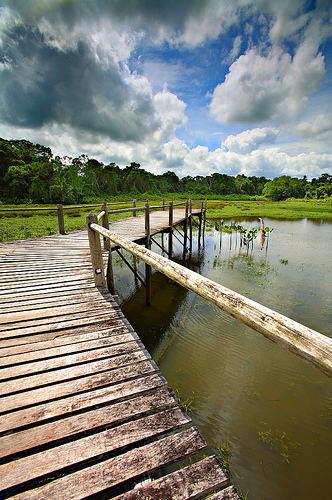
\includegraphics[width=0.06\textwidth, height=0.35in]{imggrid/datasetposi/6.jpg} &
%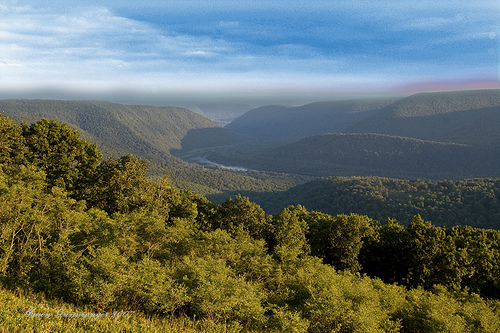
\includegraphics[width=0.06\textwidth, height=0.35in]{imggrid/datasetposi/7.jpg} &
%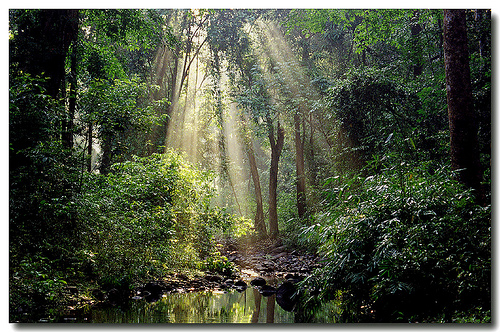
\includegraphics[width=0.06\textwidth, height=0.35in]{imggrid/datasetposi/8.jpg} &
%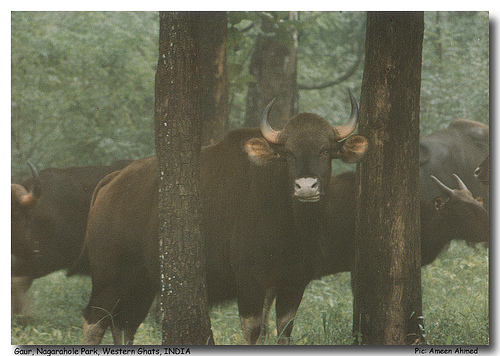
\includegraphics[width=0.06\textwidth, height=0.35in]{imggrid/datasetposi/9.jpg} &
%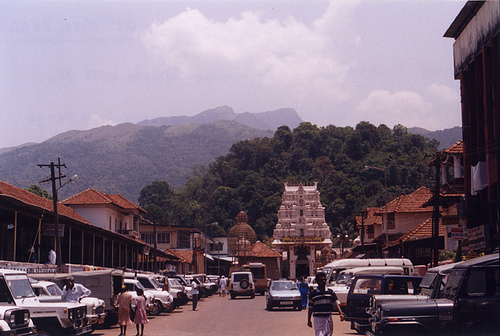
\includegraphics[width=0.06\textwidth, height=0.35in]{imggrid/datasetposi/10.jpg} \\
%\multicolumn{5}{c}{(a) Random positive images in vegetation dataset} \\ 
%\\[1pt]
%\hline
%\\[1pt]
%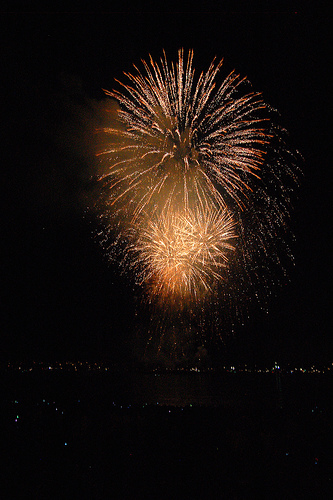
\includegraphics[width=0.06\textwidth, height=0.35in]{imggrid/datasetnega/6.jpg} &
%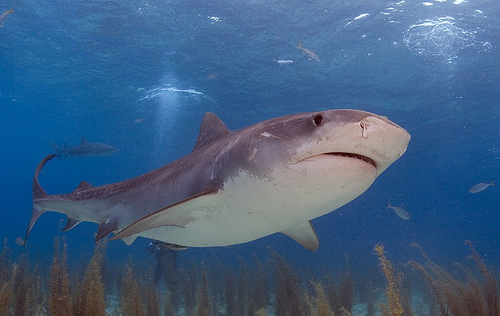
\includegraphics[width=0.06\textwidth, height=0.35in]{imggrid/datasetnega/7.jpg} &
%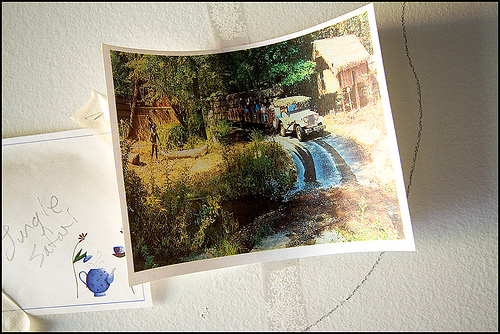
\includegraphics[width=0.06\textwidth, height=0.35in]{imggrid/datasetnega/8.jpg} &
%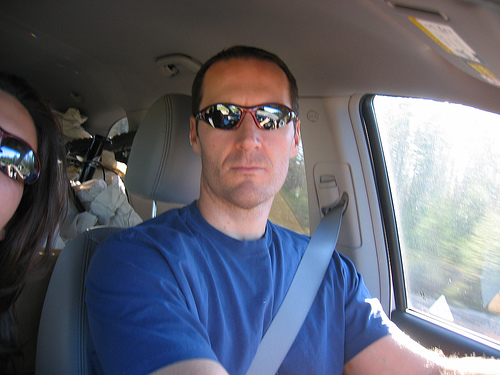
\includegraphics[width=0.06\textwidth, height=0.35in]{imggrid/datasetnega/9.jpg} &
%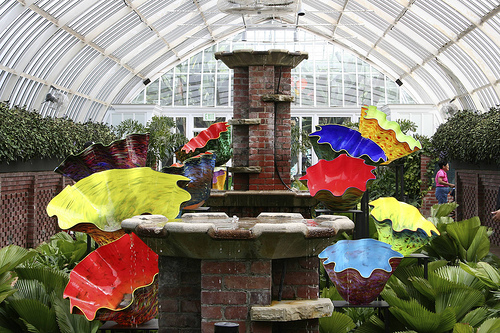
\includegraphics[width=0.06\textwidth, height=0.35in]{imggrid/datasetnega/10.jpg} \\
%\multicolumn{5}{c}{(b) Random negative images in vegetation dataset} \\
%\end{tabular}
%\end{center}
%}}
%\vspace{-6pt}
%\caption{Random images from our hand-labeled dataset. Public sharing images are various in quality, contents, illumination and view angle.
%Negative images like winter trees without leaves, or indoor images capturing a photo of forest are more confusing.}
%\label{fig:dataset}
%\end{figure}

\begin{table}[th!]
\centering
\caption {\textbf{Results of our visual models for vegetation.}}
\label{tab:veg_img_classifier} 
\tiny
\begin{tabular}{@{}cr@{}}\toprule
Visual feature &  Accuracy\\\midrule
Random Baseline & 50.00\%\\
Color SIFT & 78.10\%\\
Color GIST & 82.58\% \\
SIFT and GIST& 85.90\% \\
CNN\% &  88.00\%\\
\bottomrule
\end{tabular}
\vspace{-12pt}
\end{table}

\begin{figure}[th!]
\begin{center}
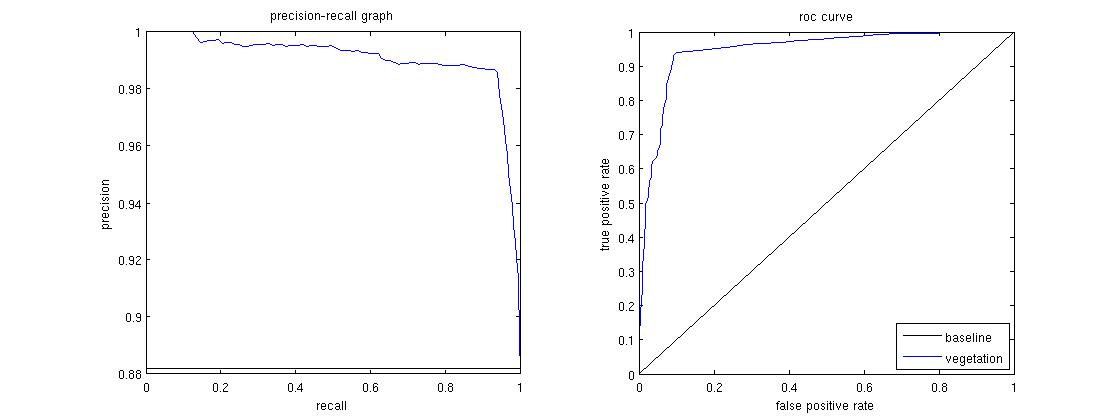
\includegraphics[width=0.4\textwidth]{figure/curvevege.jpg}
\end{center}
%}}
\vspace{-20pt}
\caption{Precision and recall curve of vegetation prediction in continental scale.}
\label{fig:curvevege}
\vspace{-12pt}
\end{figure}
%\addvspace{5mm}

%\begin{figure}[th!]
%{\tiny{
%\begin{center}
%\begin{tabular}{@{}c@{\,\,\,}c@{\,\,\,}c@{\,\,\,}c@{\,\,\,}c@{\,\,\,}}
%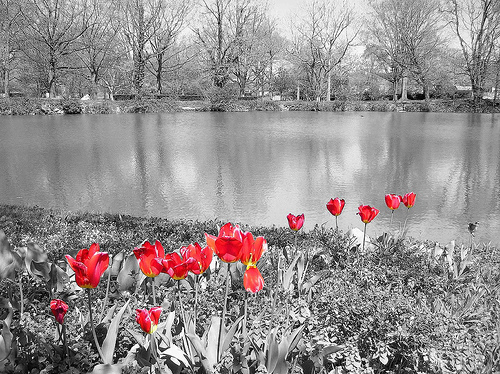
\includegraphics[width=0.06\textwidth, height=0.35in]{imggrid/falseposi/6.jpg} &
%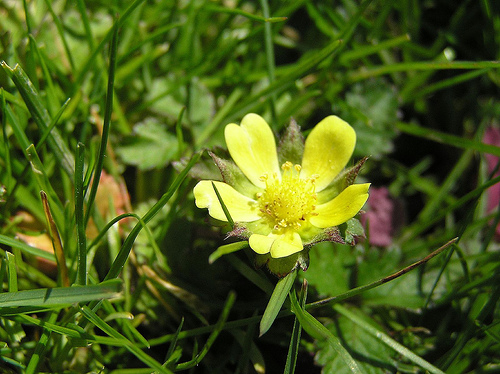
\includegraphics[width=0.06\textwidth, height=0.35in]{imggrid/falseposi/7.jpg} &
%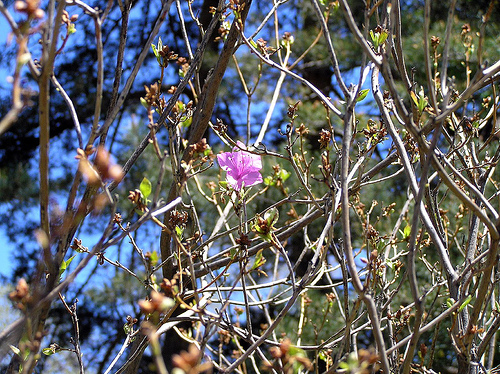
\includegraphics[width=0.06\textwidth, height=0.35in]{imggrid/falseposi/8.jpg} &
%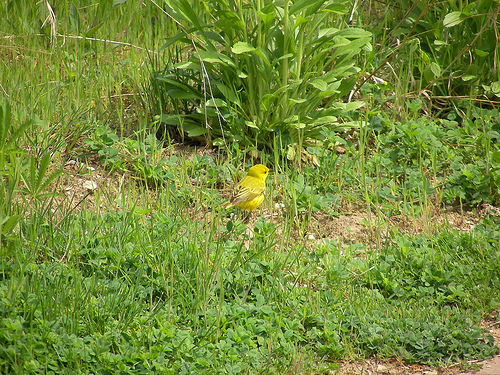
\includegraphics[width=0.06\textwidth, height=0.35in]{imggrid/falseposi/9.jpg} &
%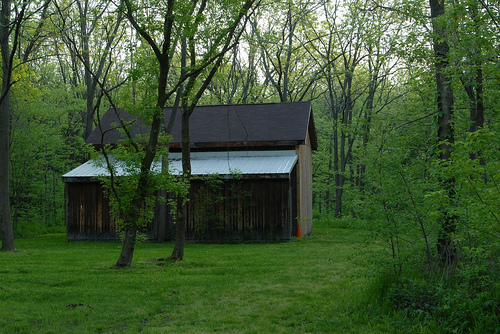
\includegraphics[width=0.06\textwidth, height=0.35in]{imggrid/falseposi/10.jpg} \\
%%\multicolumn{5}{c}{(a) Random positive images in vegetation dataset} \\ 
%\\[-6pt]
%\hline
%\\[-6pt]
%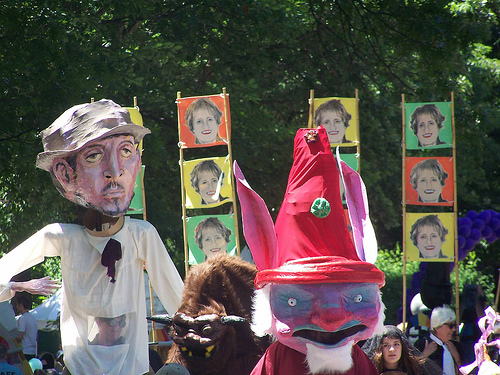
\includegraphics[width=0.06\textwidth, height=0.35in]{imggrid/falseposi/16.jpg} &
%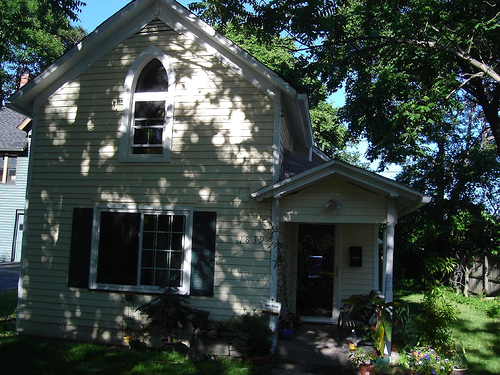
\includegraphics[width=0.06\textwidth, height=0.35in]{imggrid/falseposi/17.jpg} &
%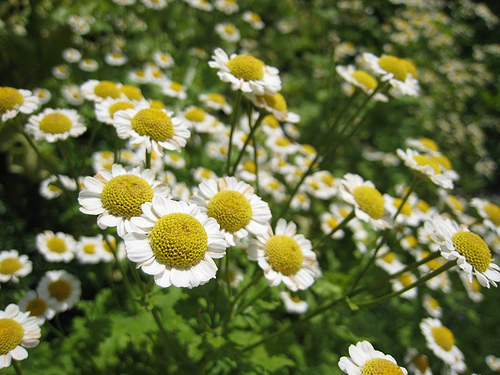
\includegraphics[width=0.06\textwidth, height=0.35in]{imggrid/falseposi/18.jpg} &
%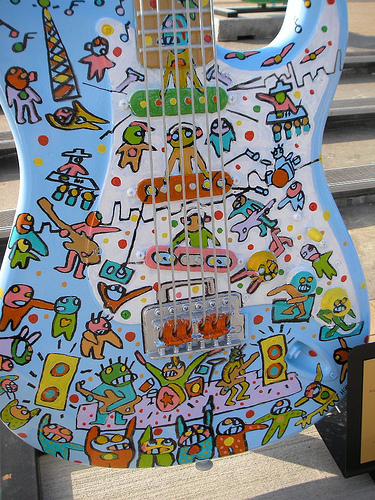
\includegraphics[width=0.06\textwidth, height=0.35in]{imggrid/falseposi/19.jpg} &
%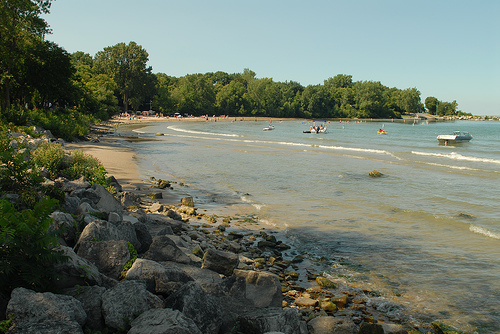
\includegraphics[width=0.06\textwidth, height=0.35in]{imggrid/falseposi/20.jpg} \\
%%\multicolumn{5}{c}{(b) Random negative images in vegetation dataset} \\
%\end{tabular}
%\end{center}
%}}
%\vspace{-6pt}
%\caption{In vegetation detection over North America in 2007, among all false positive bins, there are 47 images that are predicted as greenery. And they are the reason these bins are predicted as green. \fxnote{conclusion of very green images in non-green bin}}
%\label{fig:falseposi}
%\vspace{-6pt}
%\end{figure}

% bar plot of 2 places
\begin{figure}[th!]
%{\tiny{
\begin{center}
\begin{tabular}{ccc}
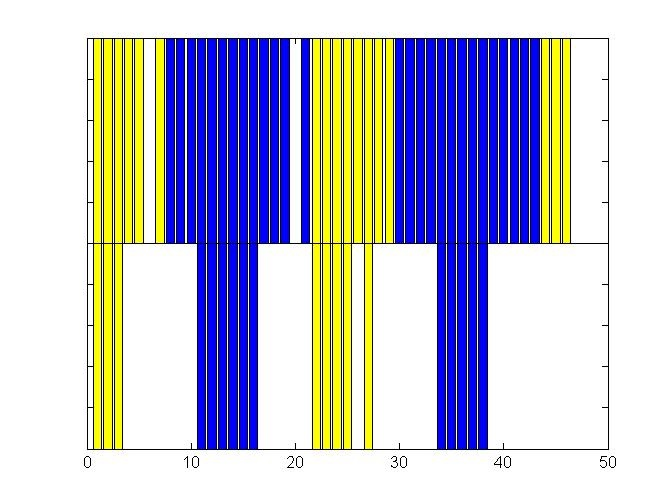
\includegraphics[width=0.14\textwidth]{bar/8560.jpg} &
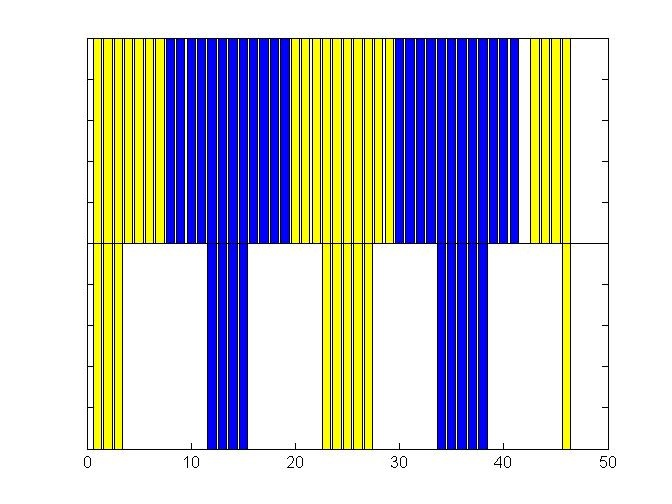
\includegraphics[width=0.14\textwidth]{bar/8561.jpg} &
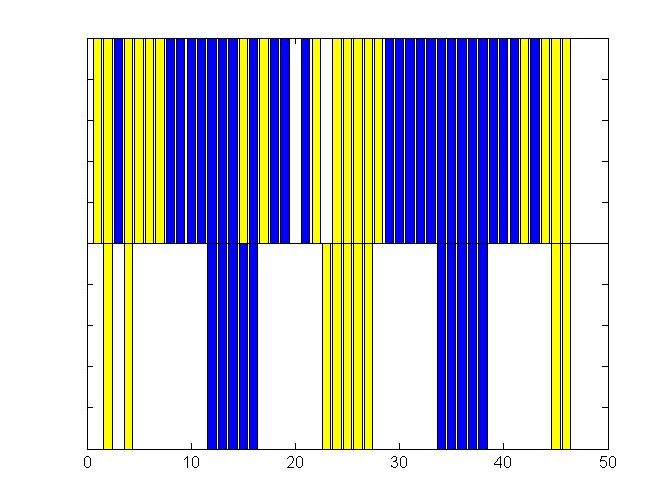
\includegraphics[width=0.14\textwidth]{bar/8881.jpg} \\
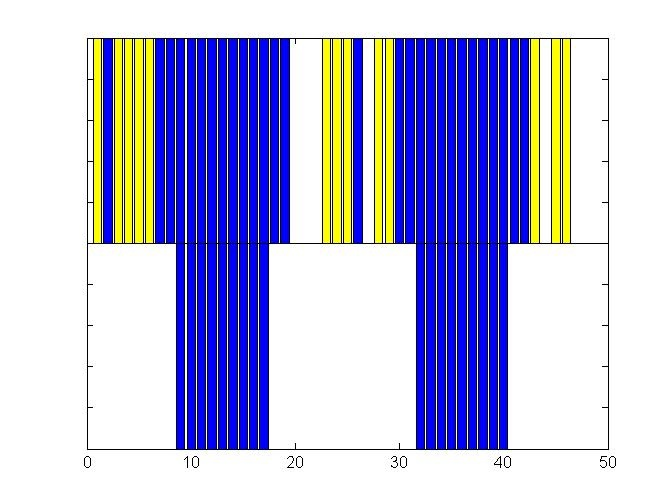
\includegraphics[width=0.14\textwidth]{bar/8911.jpg} &
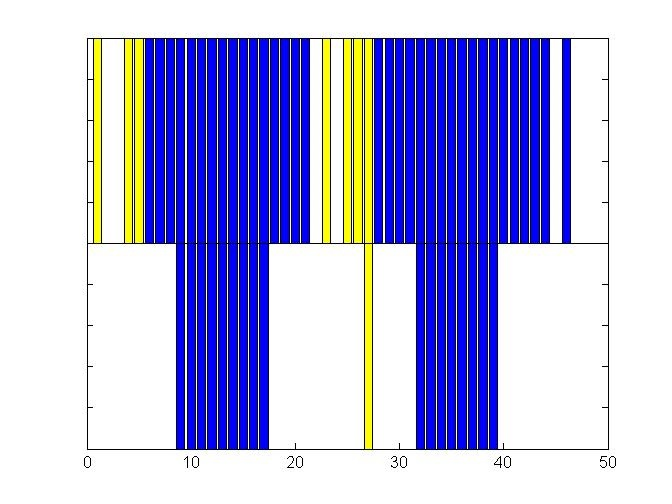
\includegraphics[width=0.14\textwidth]{bar/9705.jpg} &
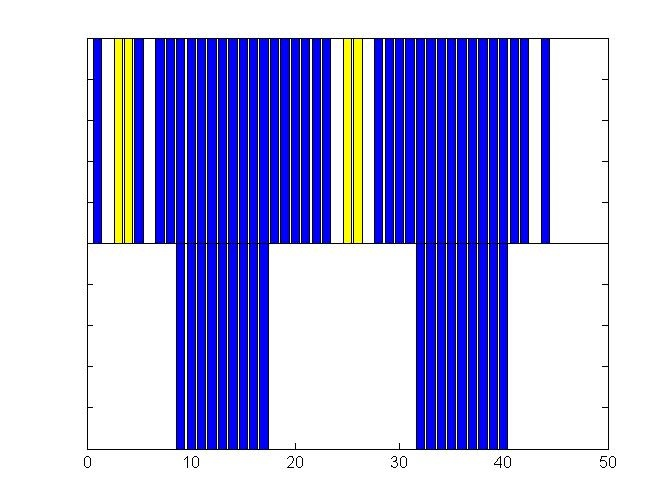
\includegraphics[width=0.14\textwidth]{bar/10816.jpg} \\
%(a) & (b)\\
\\
\end{tabular}
\end{center}
%}}
\vspace{-28pt}
\caption{Yellow bars show non-greenery at that time. Blue bars represent greenery. Prediction results on top shows 6 random places comparing to satellite ground truth. The ground truth on the bottom tends to disappear when leaves are turning yellow or green.}
\label{fig:placeinbar}
\vspace{-24pt}
\end{figure}

\begin{figure}[th!]
%{\tiny{
\begin{center}
\begin{tabular}{cccc}
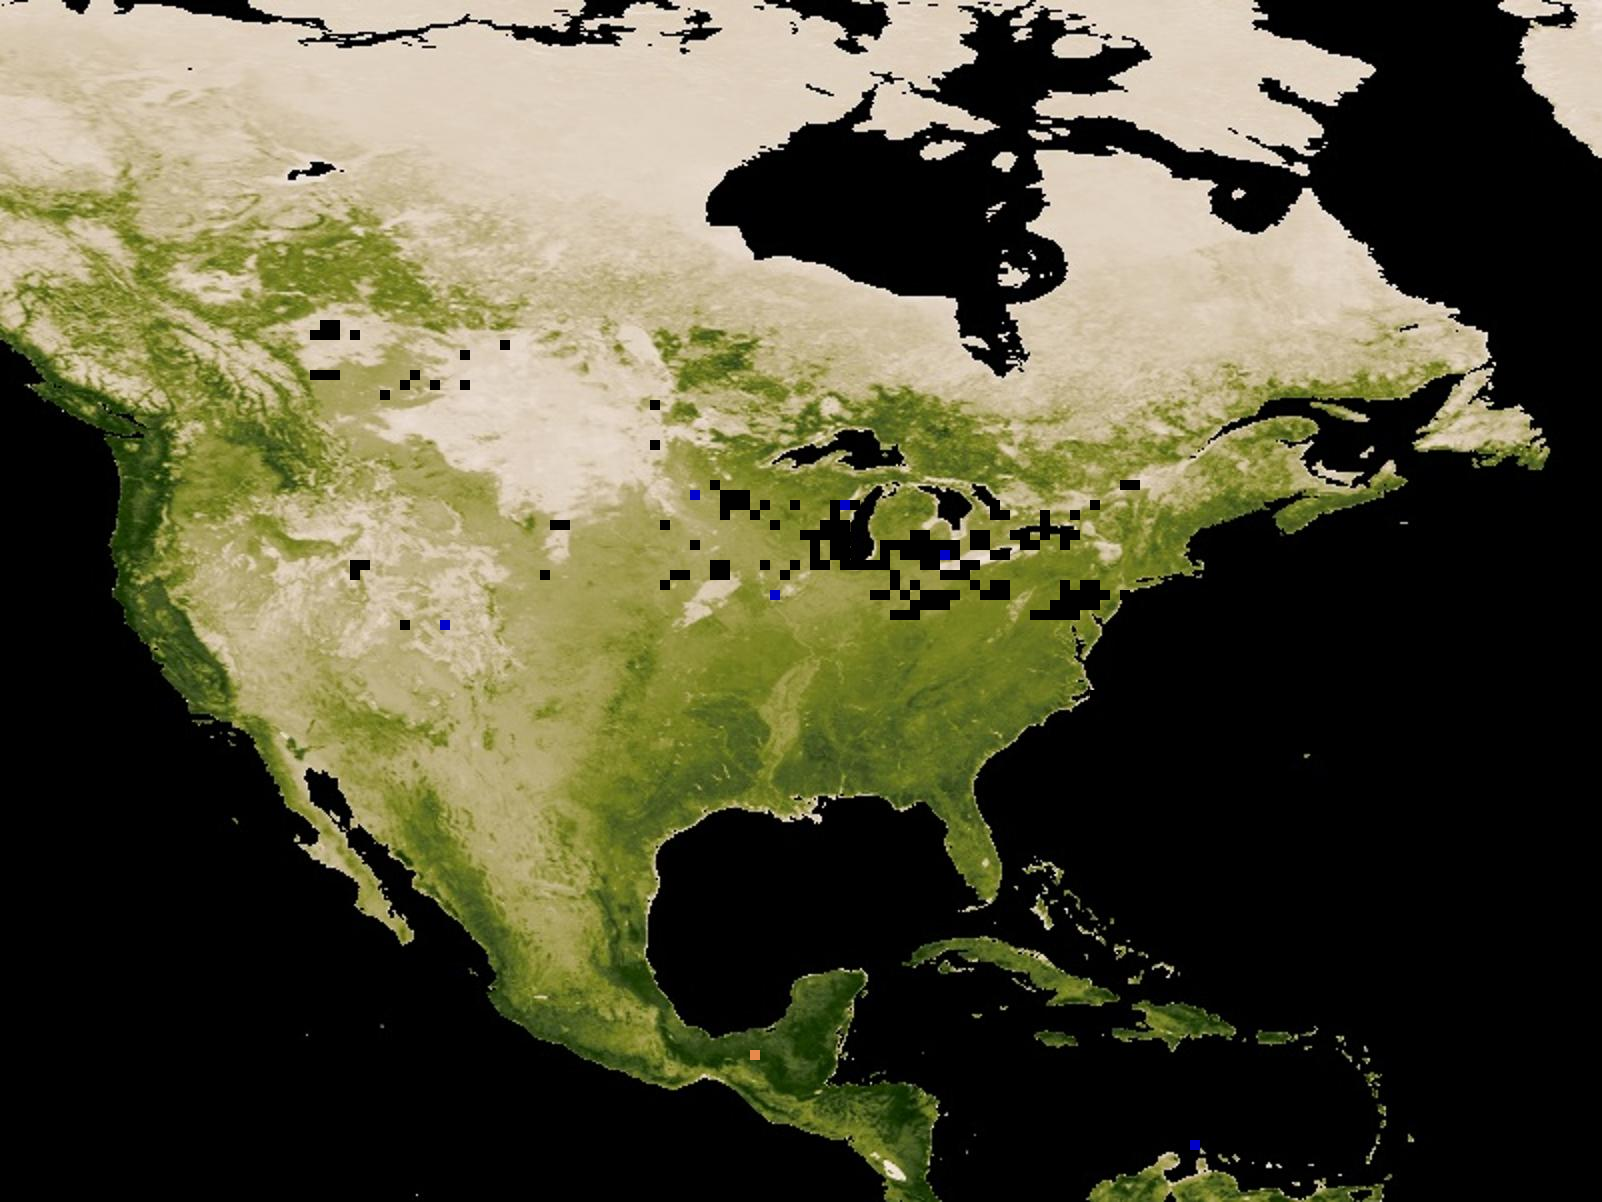
\includegraphics[width=0.10\textwidth]{map/72.png} &
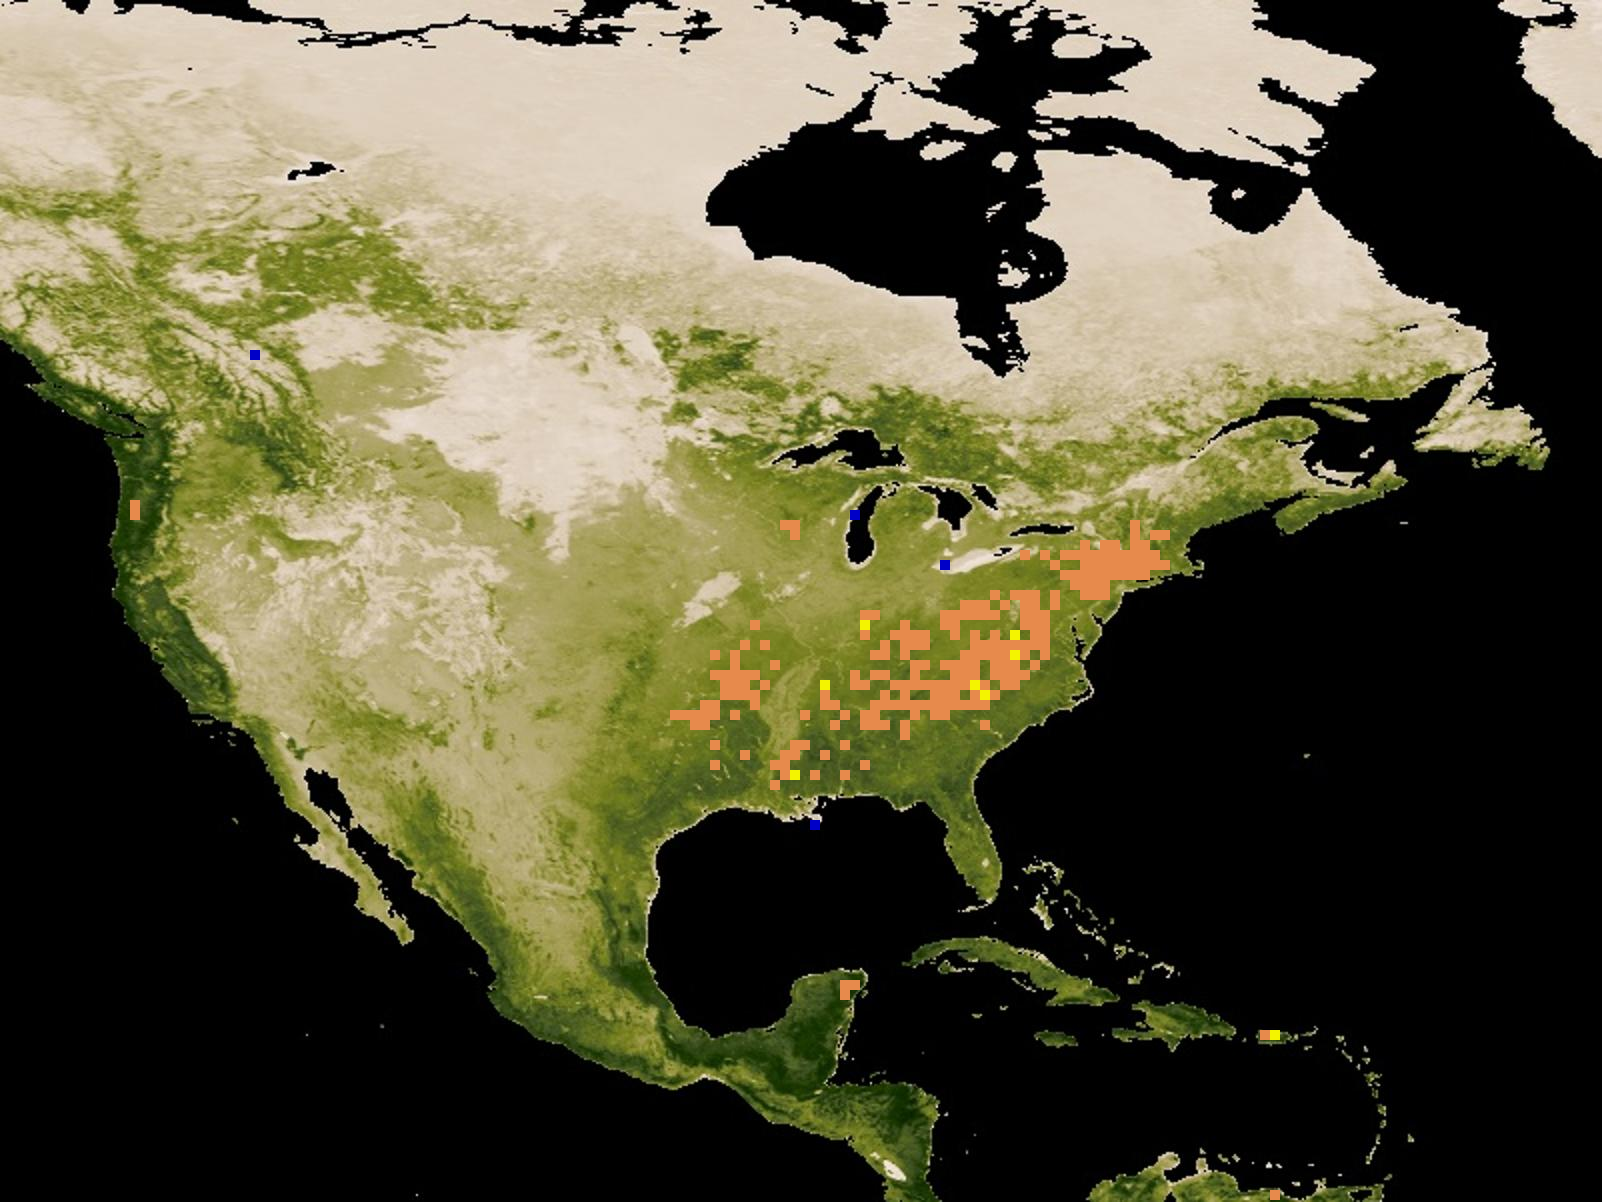
\includegraphics[width=0.10\textwidth]{map/77.png} &
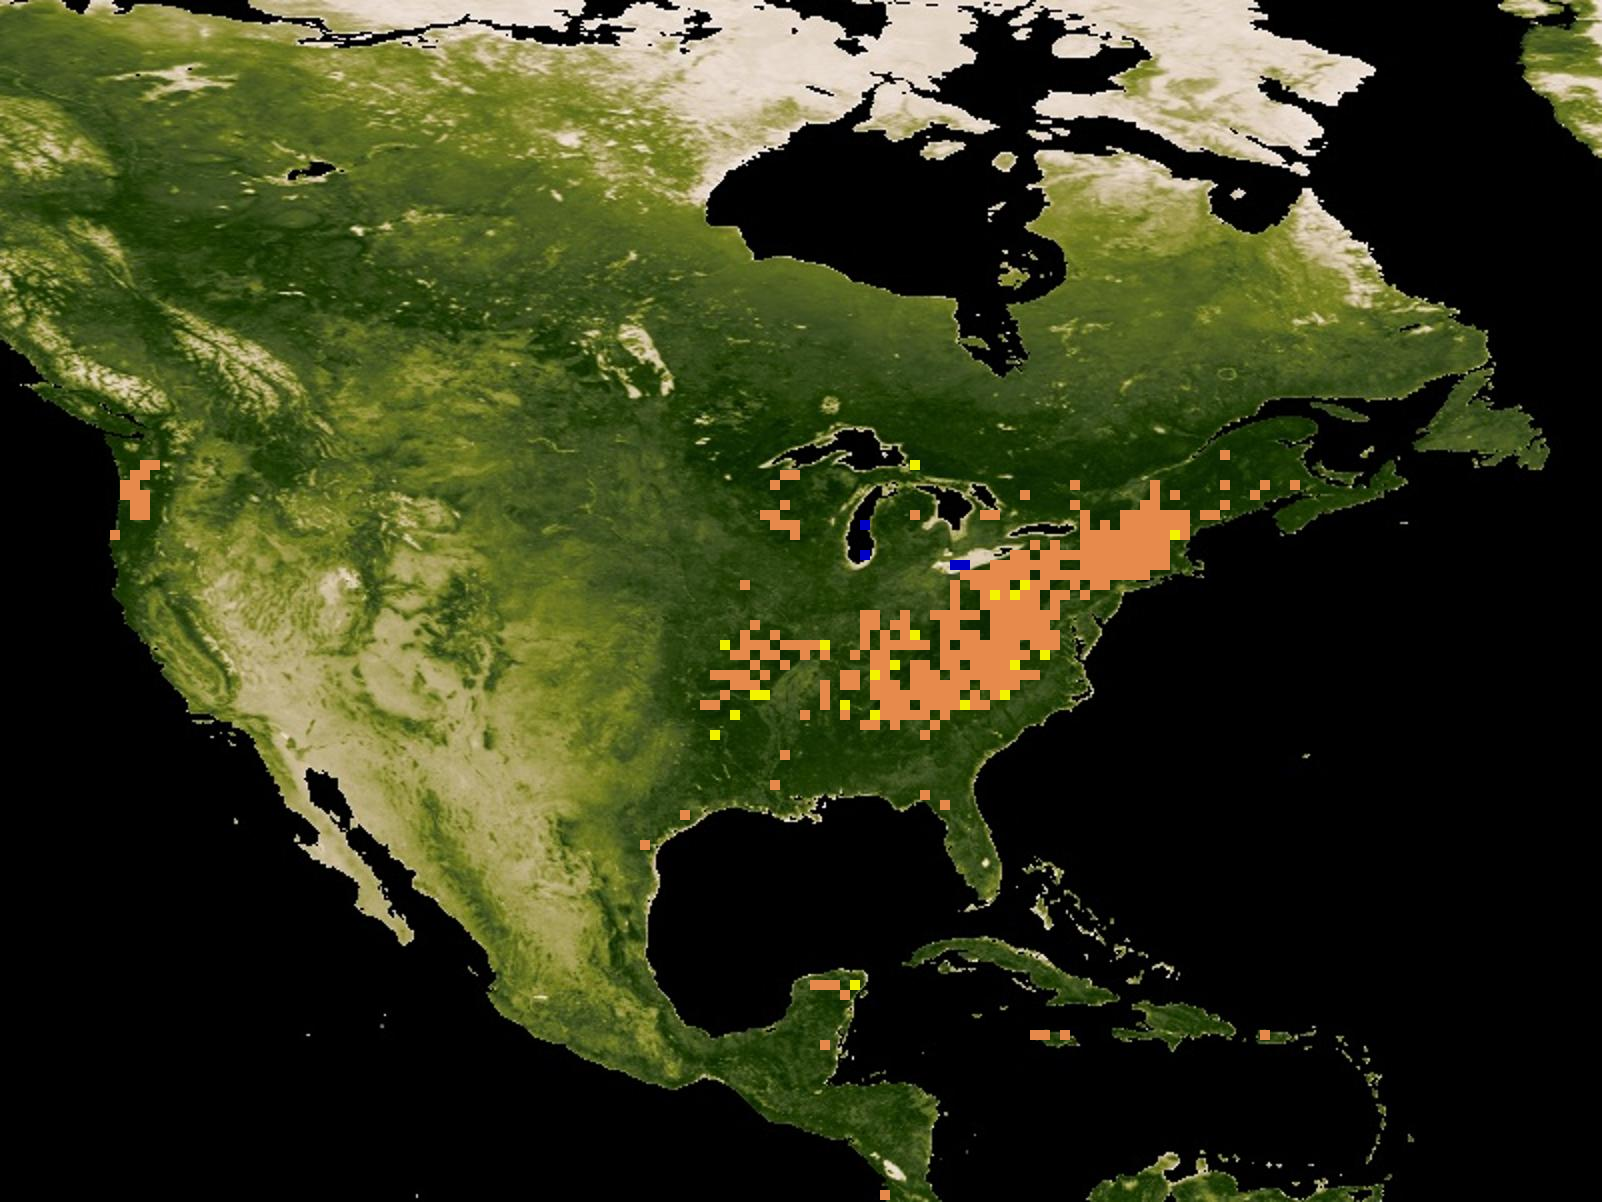
\includegraphics[width=0.10\textwidth]{map/78.png} &
%\includegraphics[width=0.5\textwidth,height=1.4in,clip,trim=0 0.5in 0in 0.6in]{plots/chicago_noaa_vs_prediction_prev_3.png} 
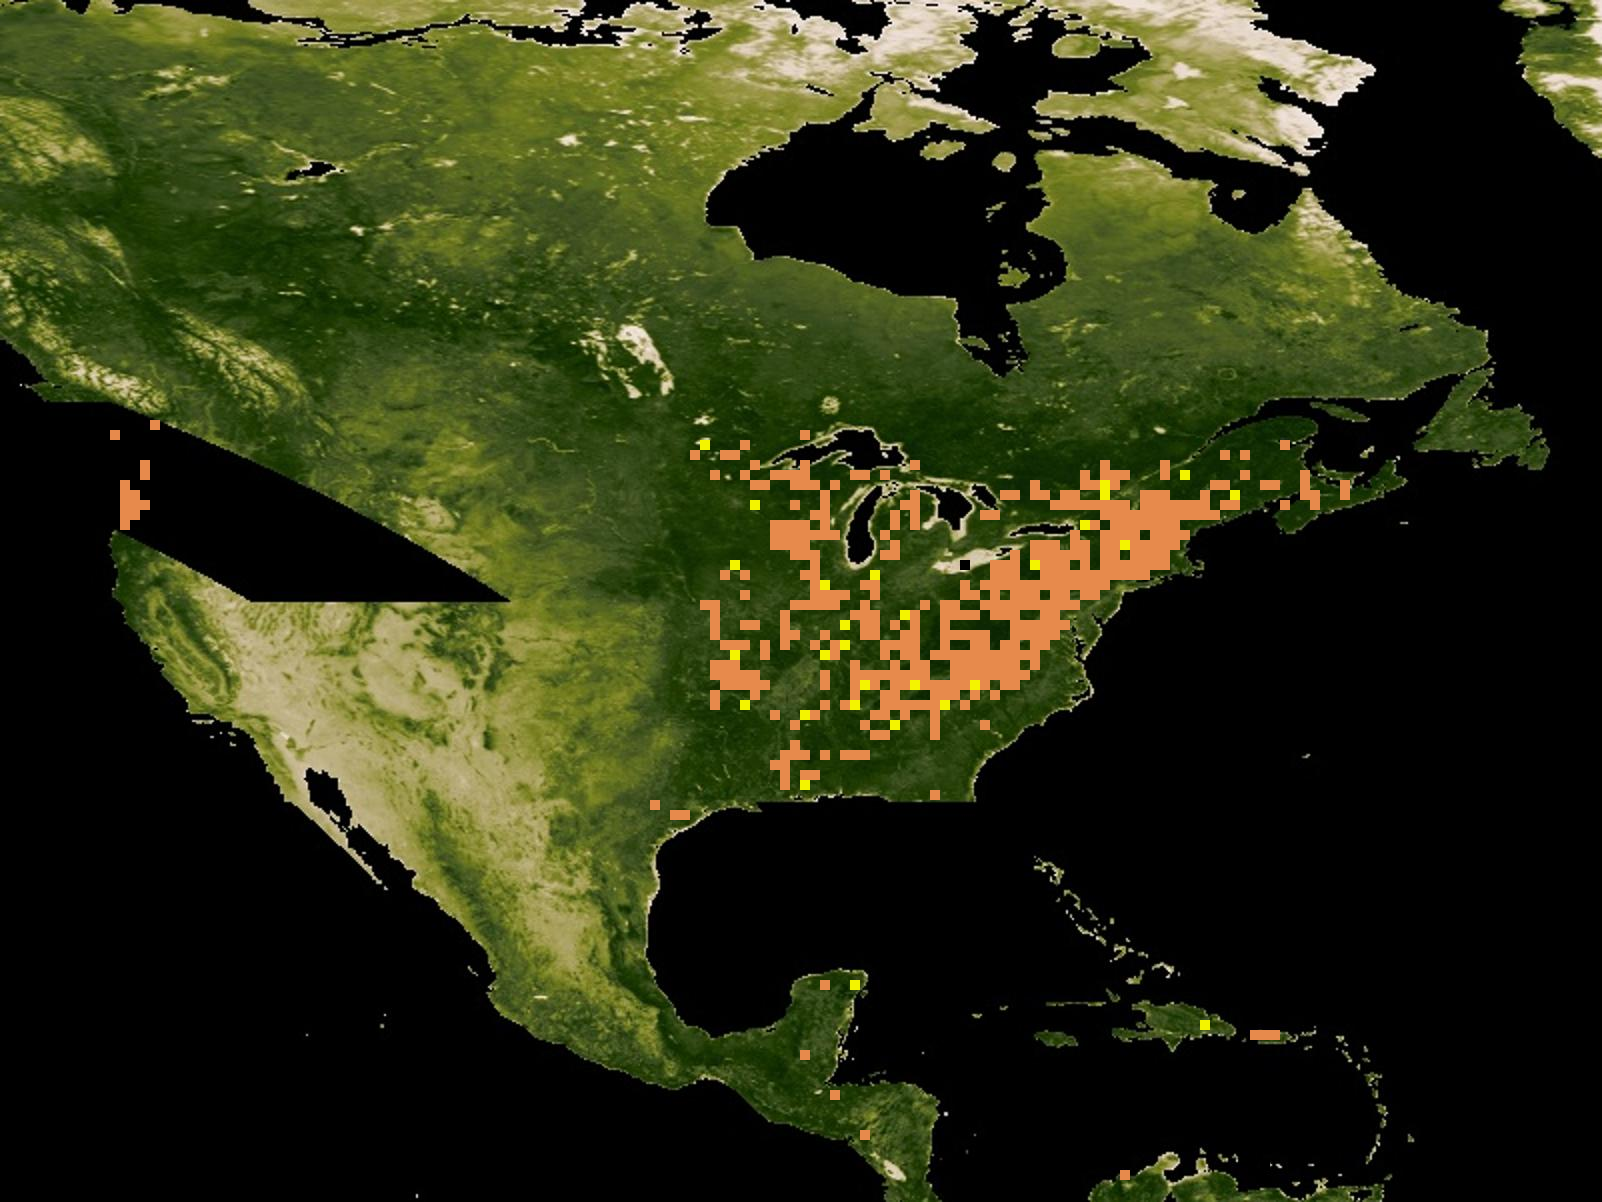
\includegraphics[width=0.10\textwidth]{map/79.png}  \\
Mar, 6th&May, 25th&Jun, 10th&Jun, 26th\\
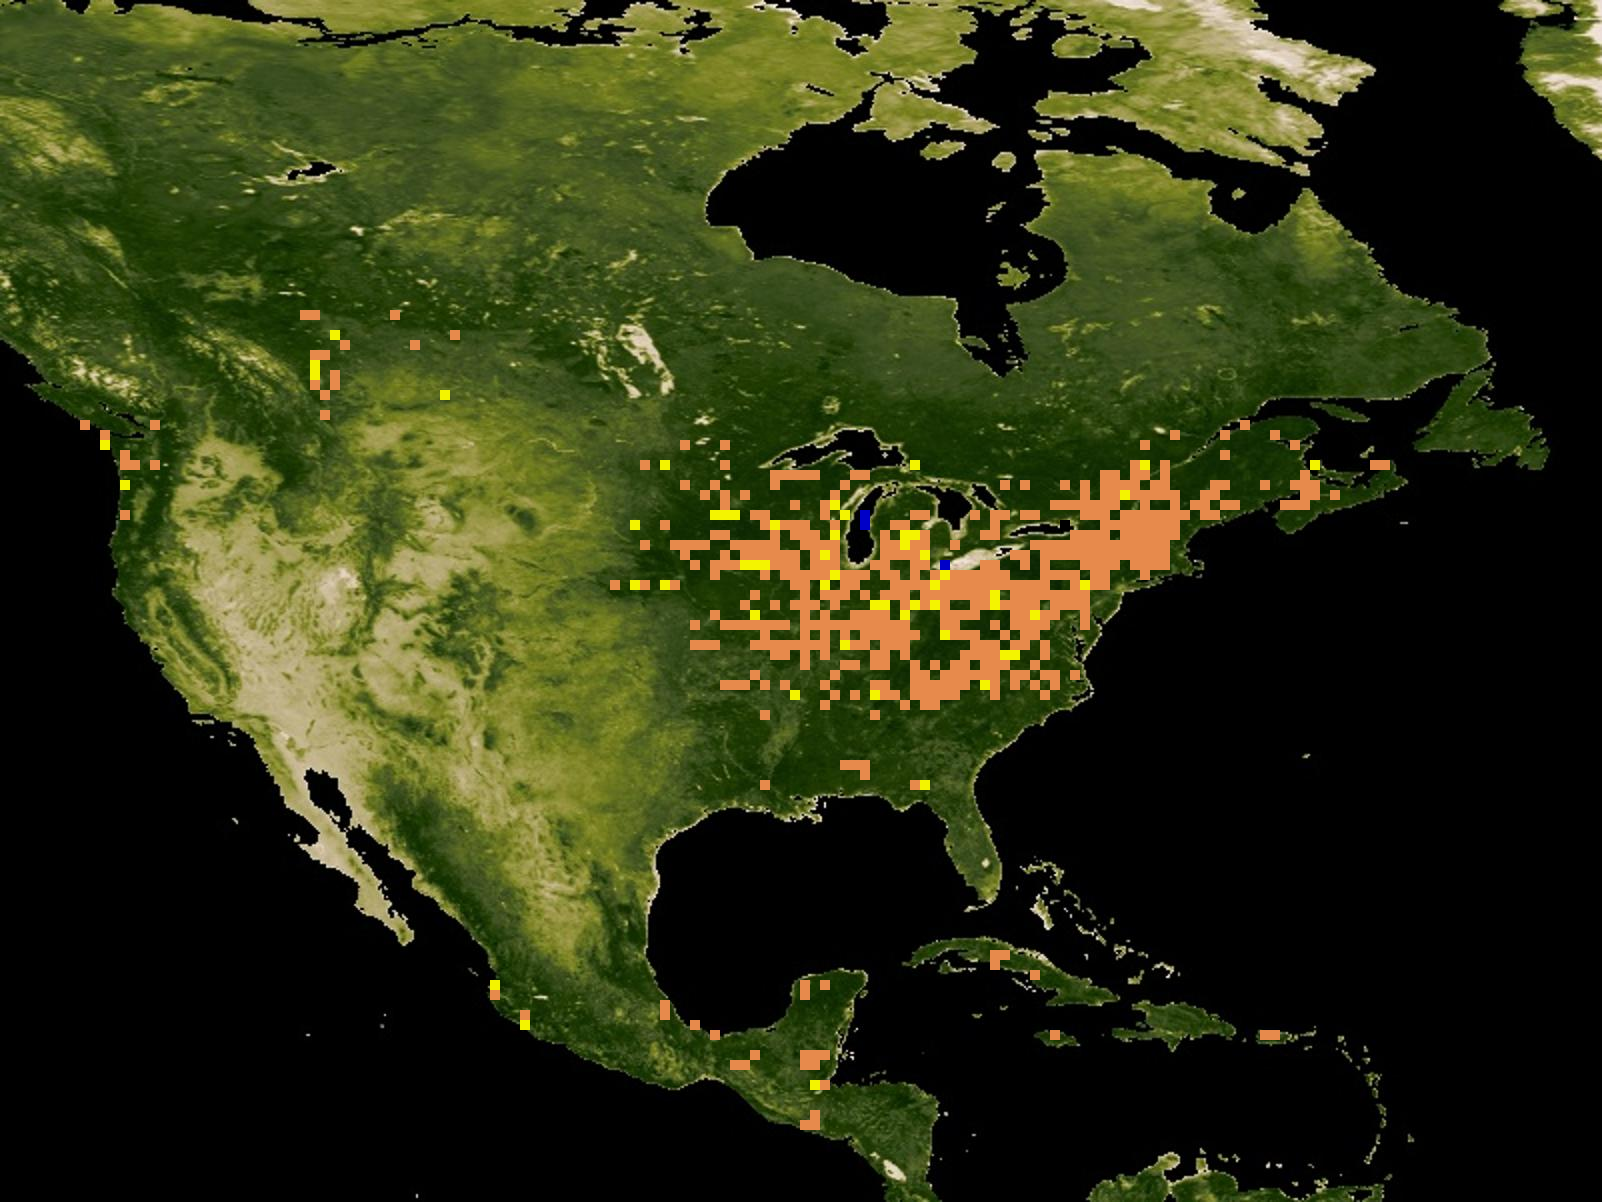
\includegraphics[width=0.10\textwidth]{map/82.png} &
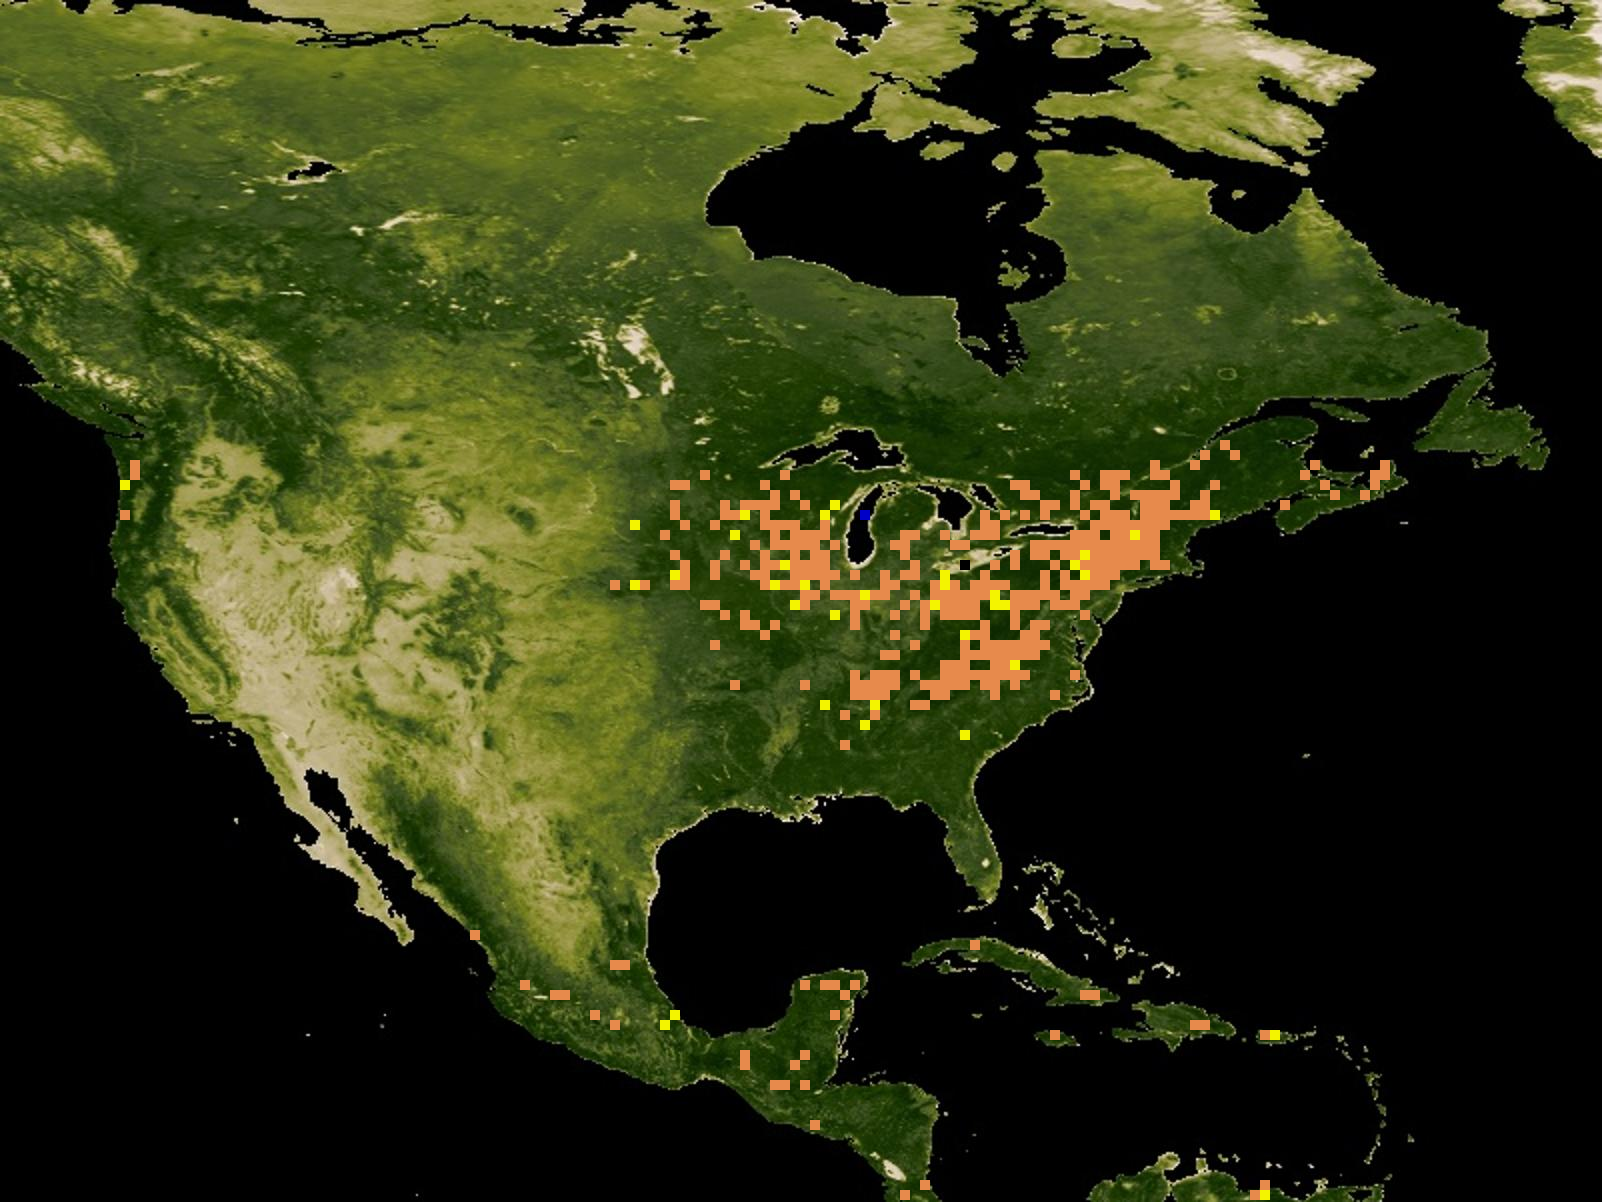
\includegraphics[width=0.10\textwidth]{map/83.png} &
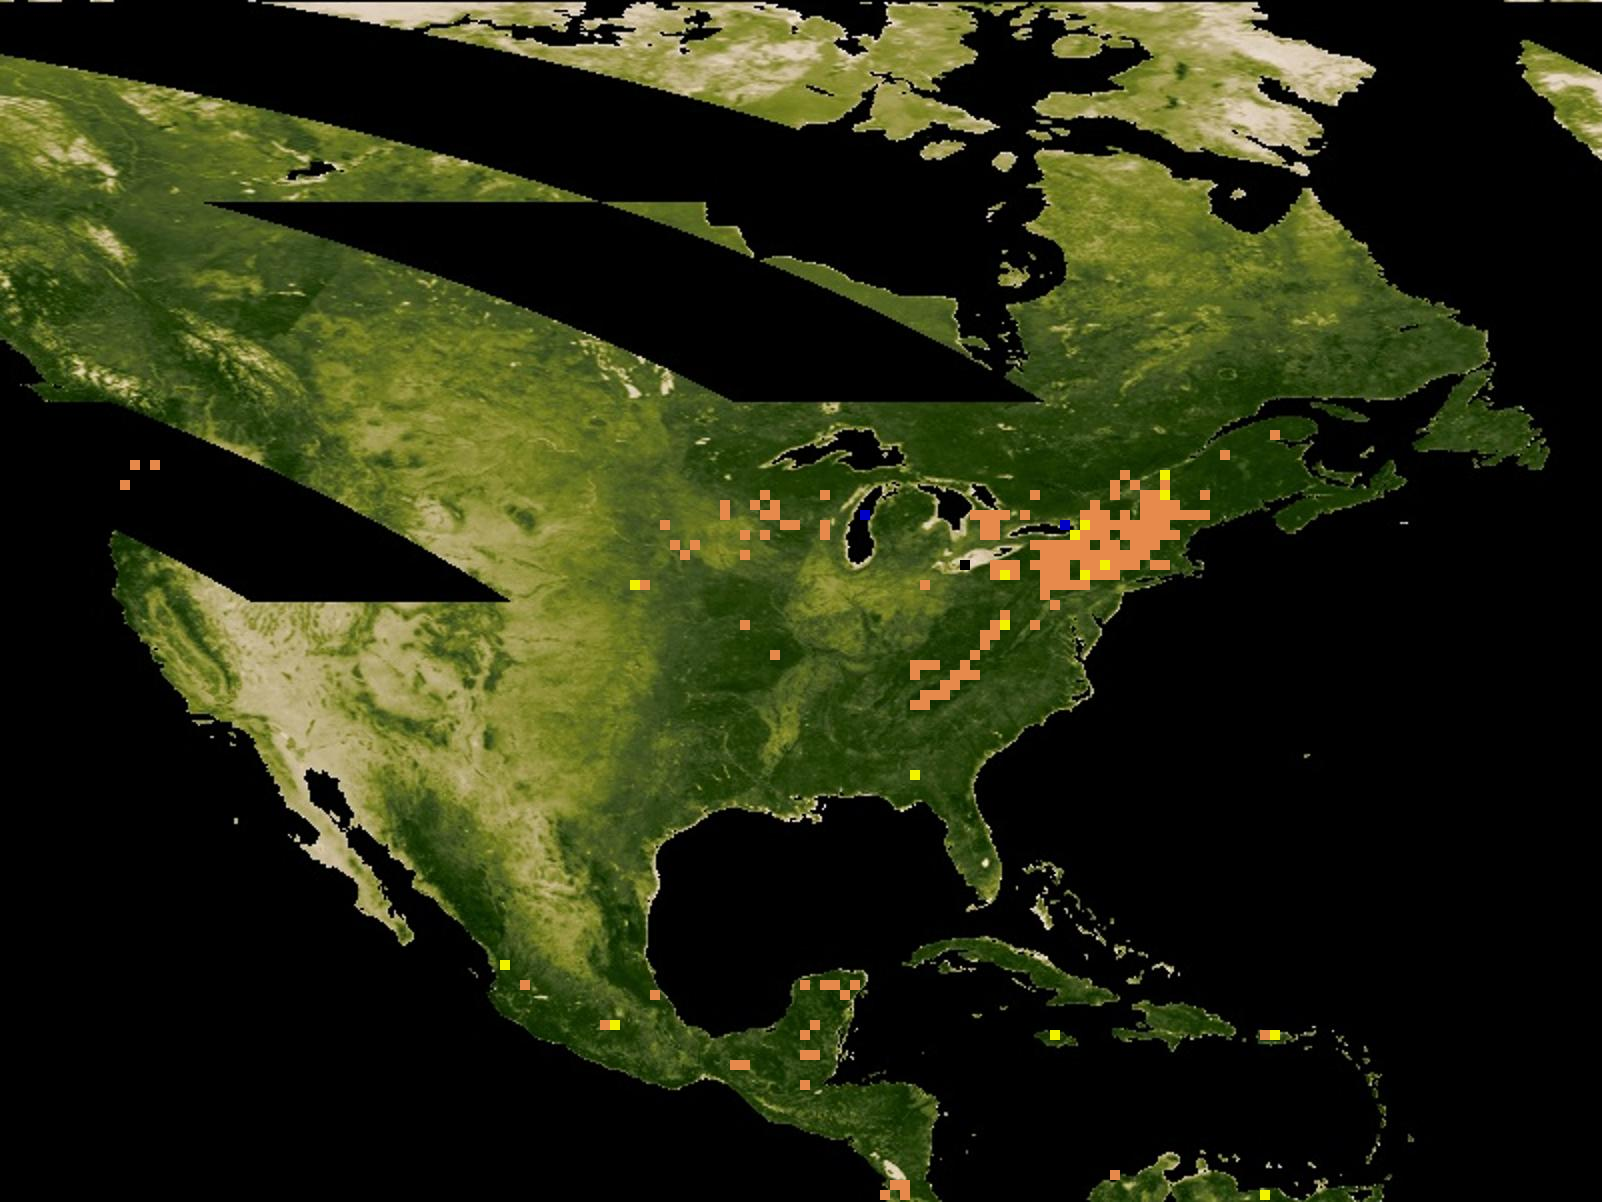
\includegraphics[width=0.10\textwidth]{map/84.png} &
%\includegraphics[width=0.5\textwidth,height=1.4in,clip,trim=0 0.5in 0in 0.6in]{plots/chicago_noaa_vs_prediction_prev_3.png} 
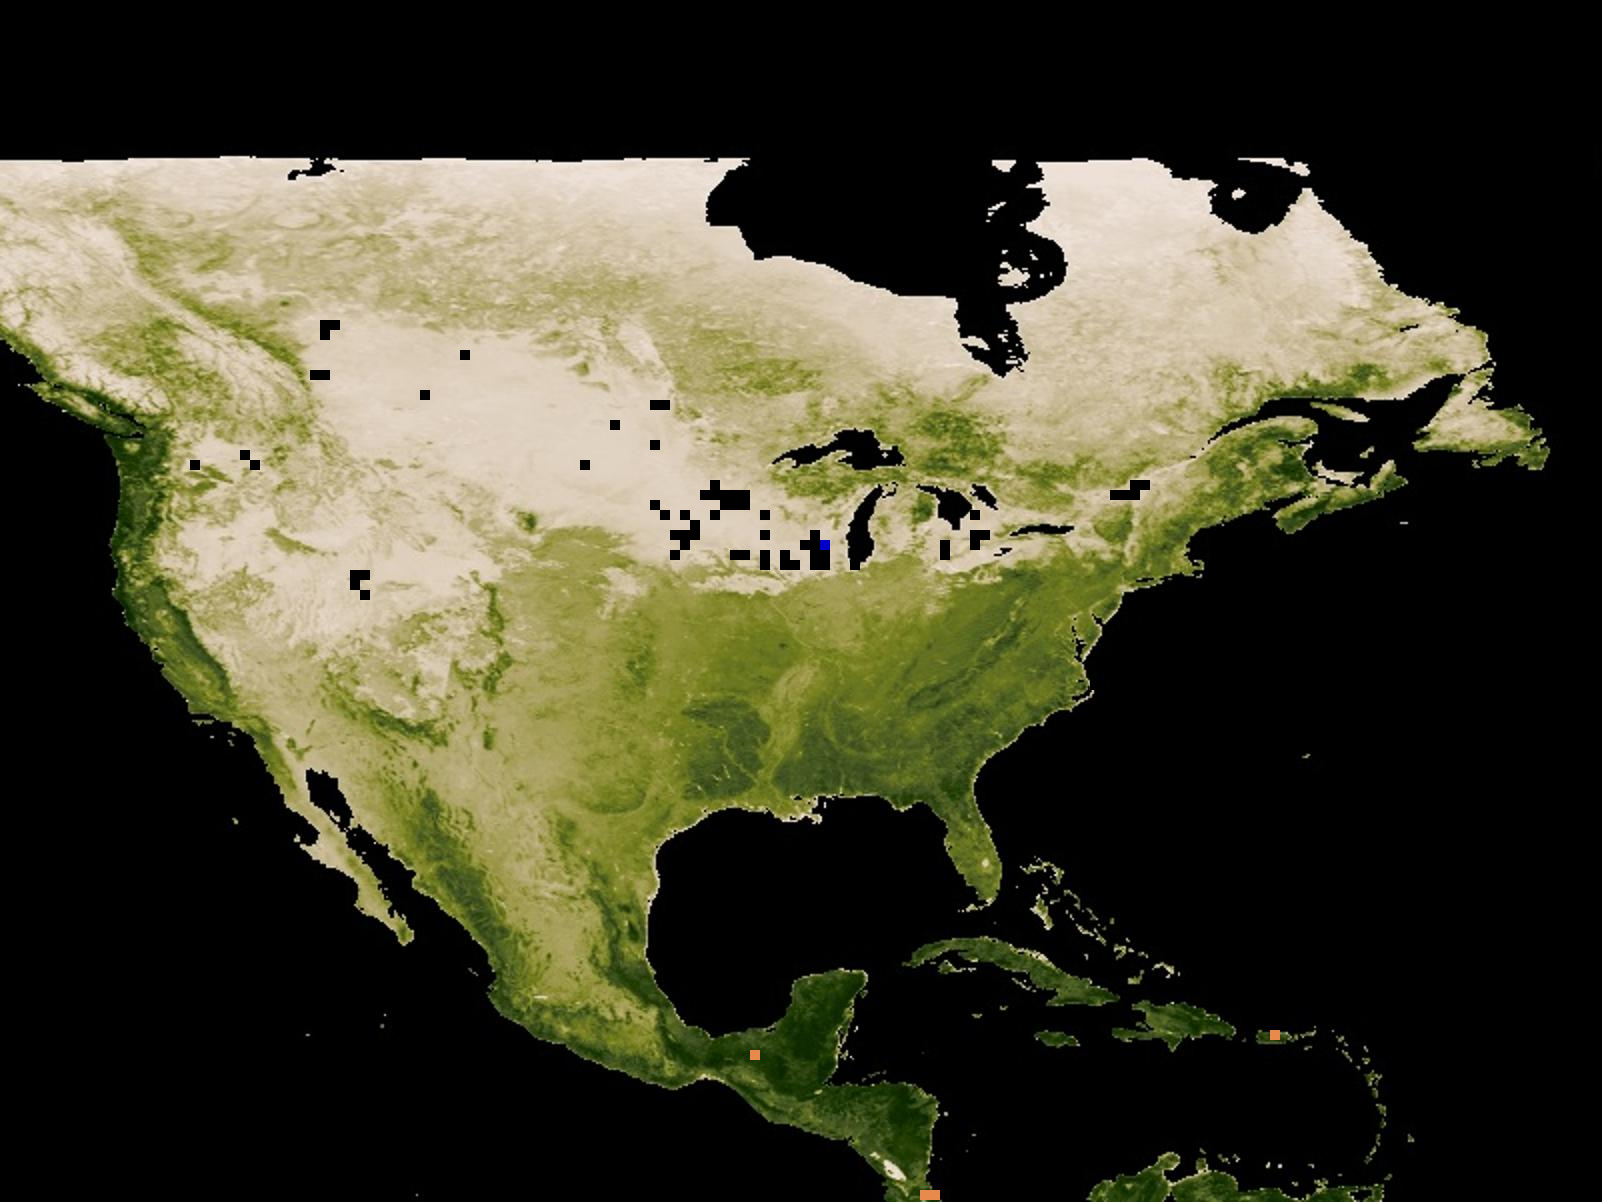
\includegraphics[width=0.10\textwidth]{map/91.png}  \\
Aug, 13th&Aug, 29th&Sep, 14th&Dec 19th\\
\\
\end{tabular}
\end{center}
%}}
\vspace{-28pt}
\caption{%On two 16-days time period, end of August on the left and during Christmas on the right, we show the confusion matrix map here. Orange bins are true positive; yellow bins are false negative; blue bins are false positive; and black bins are true negative.
We use prediction results to recreate vegetation coverage maps for each 16-days period. There are 8 maps picked in 2010. The dates under each map are the starting date of each 16-days period.
Orange bins represent true positive; blue bins are false positives; yellow bins are true negatives and black bins are false negatives. }
\label{fig:map}
\vspace{-24pt}
\end{figure}


\clearpage

%
% The following two commands are all you need in the
% initial runs of your .tex file to
% produce the bibliography for the citations in your paper.
\bibliographystyle{abbrv}
\bibliography{eco}  % sigproc.bib is the name of the Bibliography in this case

% You must have a proper ".bib" file
%  and remember to run:
% latex bibtex latex latex
% to resolve all references
%
\end{document}
